
%% =============================================================
%%  Neural LOD: Adaptive Level-of-Detail System
%%  Comprehensive Project Report
%%  COMP 432 — Learning-Based Adaptive Level-of-Detail Control
%%  Maintainer : Silent0Wings
%%  Last Updated: 2026-04-08
%% =============================================================

\documentclass[12pt, a4paper]{article}

% ── Packages ──────────────────────────────────────────────────
\usepackage[T1]{fontenc}
\usepackage[utf8]{inputenc}
\usepackage{lmodern}
\usepackage[margin=2.5cm]{geometry}
\usepackage{graphicx}
\usepackage{booktabs}
\usepackage{longtable}
\usepackage{array}
\usepackage{tabularx}
\usepackage{multirow}
\usepackage{xcolor}
\usepackage{listings}
\usepackage{hyperref}
\usepackage{amsmath}
\usepackage{amssymb}
\usepackage{float}
\usepackage{caption}
\usepackage{subcaption}
\usepackage{fancyhdr}
\usepackage{titlesec}
\usepackage{parskip}
\usepackage{enumitem}
\usepackage{mdframed}
\usepackage{tikz}
\usetikzlibrary{shapes.geometric, arrows.meta, positioning, fit, backgrounds}

% ── Colour palette ────────────────────────────────────────────
\definecolor{codeblue}{RGB}{0,90,180}
\definecolor{codegray}{RGB}{128,128,128}
\definecolor{codegreen}{RGB}{40,140,40}
\definecolor{backcolour}{RGB}{247,247,250}
\definecolor{warnorange}{RGB}{200,80,0}
\definecolor{successgreen}{RGB}{0,130,60}
\definecolor{accentblue}{RGB}{20,80,160}

% ── Listings style ────────────────────────────────────────────
\lstdefinestyle{mystyle}{
  backgroundcolor=\color{backcolour},
  commentstyle=\color{codegreen}\itshape,
  keywordstyle=\color{codeblue}\bfseries,
  numberstyle=\tiny\color{codegray},
  stringstyle=\color{warnorange},
  basicstyle=\ttfamily\footnotesize,
  breakatwhitespace=false,
  breaklines=true,
  captionpos=b,
  keepspaces=true,
  numbers=left,
  numbersep=5pt,
  showspaces=false,
  showstringspaces=false,
  showtabs=false,
  tabsize=2,
  frame=single,
  rulecolor=\color{codegray}
}
\lstset{style=mystyle}

% ── Header / Footer ───────────────────────────────────────────
\pagestyle{fancy}
\fancyhf{}
\rhead{\textcolor{accentblue}{\small Neural LOD — Project Report}}
\lhead{\small COMP 432}
\rfoot{\thepage}
\lfoot{\small Silent0Wings · 2026-04-08}

% ── Section formatting ────────────────────────────────────────
\titleformat{\section}[hang]
  {\Large\bfseries\color{accentblue}}{\thesection}{1em}{}[\titlerule]
\titleformat{\subsection}[hang]
  {\large\bfseries\color{accentblue!80!black}}{\thesubsection}{1em}{}
\titleformat{\subsubsection}[hang]
  {\normalsize\bfseries}{\thesubsubsection}{1em}{}

% ── Hyperref config ───────────────────────────────────────────
\hypersetup{
  colorlinks=true,
  linkcolor=accentblue,
  citecolor=codegreen,
  urlcolor=codeblue,
  pdftitle={Neural LOD: Adaptive Level-of-Detail System},
  pdfauthor={Silent0Wings}
}

% ── Helper box ────────────────────────────────────────────────
\newmdenv[linecolor=warnorange!70,linewidth=1pt,
  backgroundcolor=warnorange!8,
  innertopmargin=6pt,innerbottommargin=6pt]{warningbox}
\newmdenv[linecolor=successgreen!70,linewidth=1pt,
  backgroundcolor=successgreen!8,
  innertopmargin=6pt,innerbottommargin=6pt]{successbox}

% ── Graphics path ─────────────────────────────────────────────
% Paths are relative to the TEX file location.
% Adjust if compiling from a different working directory.
\graphicspath{
  {../../plots/}
  {../../plots/Stage_1/}
  {../../plots/Stage_2/}
  {../../plots/Stage_2_2/}
  {../../plots/Stage_3/}
  {../../plots/Stage_4/}
  {../../plots/training/}
  {../../Diagram/Stage_1/}
  {../../Diagram/Stage_2/}
  {../../Diagram/Stage_3/}
  {../../Diagram/Stage_4/}
}

% =============================================================
\begin{document}

% ── Title page ────────────────────────────────────────────────
\begin{titlepage}
  \centering
  \vspace*{2cm}
  {\Huge\bfseries\color{accentblue} Neural LOD}\\[0.4cm]
  {\LARGE Adaptive Level-of-Detail System}\\[0.3cm]
  {\large\color{codegray} Learning-Based Real-Time LOD Control in Unity}\\[2cm]
  \rule{0.8\textwidth}{0.5pt}\\[1cm]
  {\large\bfseries Course:} COMP 432\\[0.3cm]
  {\large\bfseries Repository:} \url{https://github.com/Silent0Wings/neural-lod}\\[0.3cm]
  {\large\bfseries Author:} Silent0Wings\\[0.3cm]
  {\large\bfseries Date:} April 8, 2026\\[1cm]
  \rule{0.8\textwidth}{0.5pt}\\[1cm]
  \begin{abstract}
    \noindent
    This report documents the full design, implementation, and evaluation of
    \textbf{Neural LOD} — a machine-learning system that trains neural networks
    to predict optimal Level-of-Detail (LOD) thresholds for real-time rendering
    inside a Unity scene. The system progresses through four training stages,
    evolving from a scalar global bias predictor (Stage~1) to a per-object
    threshold vector predictor (Stage~3) to a REINFORCE reinforcement-learning
    policy (Stage~4). Data are collected by automated Unity playback, labelled
    with a reactive oracle, and fed to PyTorch MLP models exported as ONNX for
    Unity inference via \texttt{com.unity.ai.inference}. The best v4 model
    achieves \textbf{MAE\,=\,0.039} bias units and reduces over-budget frames
    from 55.2\,\% (fixed baseline) to \textbf{47.5\,\%} at runtime. Stability
    filters (EMA + dwell timer) eliminate previously observed LOD jitter.
  \end{abstract}
  \vfill
  {\small Status: Active Development — Stages 1–4 Complete}
\end{titlepage}

% ── Table of contents ─────────────────────────────────────────
\tableofcontents
\newpage

% =============================================================
\section{Project Overview}
\label{sec:overview}

\subsection{Motivation}

Real-time 3D applications continuously balance visual quality against rendering
budget. Unity's built-in LOD system transitions between pre-authored mesh
resolutions based on a single global parameter — \texttt{QualitySettings.lodBias}
— or on static per-object screen-relative thresholds. Neither approach adapts to
\emph{runtime context}: camera speed, scene density, spatial zone, and available
GPU headroom all affect the optimal trade-off, yet the engine ignores them.

Neural LOD replaces these static policies with neural networks that learn the
optimal decision per frame from real gameplay telemetry. The trained models are
deployed as ONNX assets and run inside Unity via the official AI Inference engine.

\subsection{System Architecture}

The project is structured as three strictly isolated subsystems (cross-subsystem
file access is forbidden by the repository rules):

\begin{description}[leftmargin=2cm, labelwidth=1.8cm]
  \item[\texttt{/ml\_pipeline}] Python pipeline: data merging, oracle labelling,
    model training (PyTorch), ONNX export, evaluation.
  \item[\texttt{/Assets}] Unity project: C\# logging scripts, inference controllers,
    deployed ONNX models and scaler JSON.
  \item[\texttt{/LLM\_Integration}] Optional orchestration layer for complex
    automated workflows.
\end{description}

\subsection{Stage Progression}

\begin{table}[H]
\centering
\caption{Project stages and key results}
\label{tab:stages}
\begin{tabularx}{\textwidth}{c X X c}
\toprule
\textbf{Stage} & \textbf{Description} & \textbf{Key Result} & \textbf{Status}\\
\midrule
0 & Verify proposal alignment & All promises delivered & \textcolor{successgreen}{\checkmark}\\
1 & Dynamic scalar \texttt{lodBias} predictor & MAE\,=\,0.039, full range & \textcolor{successgreen}{\checkmark}\\
2 & Per-object baker threshold predictor & P99\,=\,18.37\,ms, FPS\,$\approx$101 & \textcolor{successgreen}{\checkmark}\\
3 & 4-value threshold vector predictor & Independent per-LOD-level control & \textcolor{successgreen}{\checkmark}\\
4 & REINFORCE RL policy + stability filters & Jitter eliminated, 0.76\,\% switch rate & \textcolor{successgreen}{\checkmark}\\
\bottomrule
\end{tabularx}
\end{table}

% =============================================================
\section{Data Collection \& Storage}
\label{sec:data}

\subsection{Unity Logging Infrastructure}

All telemetry originates from \texttt{MetricLogger.cs} running inside the Unity
Editor/build. The logger is driven by \texttt{DataCollectionOrchestrator.cs},
which sweeps every combination of \texttt{biasValues} $\times$ \texttt{moveSpeeds}
$\times$ \texttt{rotateSpeeds}, collecting a fixed row cap per run (default 5000).

Key implementation choices that shaped data quality:

\begin{itemize}
  \item \textbf{Deterministic camera path:} \texttt{CameraPathAnimator.cs} uses
    waypoint-based child \texttt{Transform} nodes, exposing \texttt{PathProgress}
    (float) and \texttt{CurrentIndex} for labelling.
  \item \textbf{Frame timing:} \texttt{FrameTimingManager} supplies
    \texttt{cpuFrameTime} and \texttt{gpuFrameTime} per interval; a
    \texttt{ProfilerRecorder} captures triangle count, draw calls, batches, and
    SetPass calls.
  \item \textbf{Frustum coverage:} Visible renderer count and mean screen coverage
    are computed via \texttt{GeometryUtility.TestPlanesAABB} with a
    \emph{pre-allocated} \texttt{Plane[6]} field (non-allocating overload) to
    eliminate per-frame GC allocations; sampled every 30 frames after profiler
    analysis identified the coverage pass as the top CPU spike.
  \item \textbf{Row cap:} Configurable \texttt{targetRowCount} (default 5000);
    sets \texttt{loggingComplete = true} and triggers \texttt{RunTerminator.cs}
    for graceful shutdown.
\end{itemize}

\subsection{CSV Schema}

The logged CSV contains 24 columns used both for training and for evaluation
parity checks. Table~\ref{tab:csv_schema} lists the key columns.

\begin{longtable}{l l p{7cm}}
\caption{Training CSV column schema (24 columns total)}\label{tab:csv_schema}\\
\toprule
\textbf{Column} & \textbf{Type} & \textbf{Notes}\\
\midrule
\endfirsthead
\toprule
\textbf{Column} & \textbf{Type} & \textbf{Notes}\\
\midrule
\endhead
\bottomrule
\endfoot
\texttt{cpu\_frame\_time\_ms} & float & Primary bottleneck signal\\
\texttt{gpu\_frame\_time\_ms} & float & Secondary bottleneck signal\\
\texttt{triangle\_count} & int & Geometric load proxy\\
\texttt{camera\_velocity} & float & Linear camera speed\\
\texttt{camera\_angular\_velocity} & float & Rotation rate (deg/s)\\
\texttt{visible\_renderer\_count} & int & Frustum complexity\\
\texttt{lod\_bias\_current} & float & Controller state at time of logging\\
\texttt{fps} & float & Derived from \texttt{deltaTime}\\
\texttt{draw\_call\_estimate} & int & \texttt{ProfilerRecorder} output\\
\texttt{previous\_bias} & float & Prior controller state\\
\texttt{frame\_headroom\_ms} & float & $16.6 - \texttt{cpu\_frame\_time\_ms}$\\
\texttt{cam\_pos\_x/y/z} & float & World-space camera position\\
\texttt{cam\_rot\_y} & float & Camera yaw angle\\
\texttt{screen\_coverage} & float & Mean per-object screen area\\
\texttt{move\_speed} & float & Run parameter (training only)\\
\texttt{rotate\_speed} & float & Run parameter (training only)\\
\texttt{waypoint\_index} & int & Current path node\\
\texttt{path\_progress} & float & Continuous 0–1 path position\\
\texttt{draw\_calls} & int & Supplemental draw-call count\\
\texttt{batches\_count} & int & Additional feature\\
\texttt{setpass\_calls} & int & Additional feature\\
\texttt{target\_lod\_bias} & float & \textbf{Oracle label (output target)}\\
\end{longtable}

\subsection{Data Volumes and Organisation}

\begin{itemize}
  \item \textbf{Stage 1 training:} 135,000 rows from 27 CSV runs across
    bias $\in \{0.25, 1.0, 2.0\}$ at multiple camera speeds.
  \item \textbf{Stage 2 baker:} 43,200 samples (10,800 after per-pose aggregation)
    from the Baker scene at 4 camera positions $\times$ rotation grid.
  \item \textbf{Stage 4 RL rollouts:} 56,024 rows (improved larger dataset) with
    15.5\,\% non-zero actions, balanced floor/ceiling dwell coverage.
\end{itemize}

Raw CSVs are stored in \texttt{ml\_pipeline/data/Train\_Runs/} and treated as
\textbf{READ-ONLY} by pipeline rules. Merged and labelled outputs land in
\texttt{data/Train\_Merged\_Unlabeled/} and \texttt{data/Train\_Merged\_labeled/}
respectively.

\subsection{Known Data Issue: CPU-Flat Scene}

\begin{warningbox}
\textbf{CPU-Flat Scene (Section 2.3.1).}
\texttt{cpu\_frame\_time\_ms} is nearly identical (\textasciitilde16.65–16.75\,ms)
across ALL bias levels. The scene is CPU-bound by non-LOD work (scripting,
physics, logging overhead). LOD bias does not move the CPU bottleneck.
\textbf{Resolution:} The oracle was switched to use \texttt{gpu\_frame\_time\_ms}
as the budget signal (\texttt{GPU\_BUDGET\_MS\,=\,4.0\,ms}), which does scale with
bias (\textasciitilde1.0\,ms spread). This is not a controller failure — the
neural controller correctly identifies the CPU-bound bottleneck and responds to
the GPU signal instead.
\end{warningbox}

% =============================================================
\section{ML Pipeline: Training \& Evaluation Logic}
\label{sec:ml}

\subsection{Pipeline Orchestration}

All pipeline stages are driven by \texttt{ml\_pipeline/run\_pipeline.py}:

\begin{lstlisting}[language=bash, caption=Pipeline invocation examples]
# Run all stages sequentially
python ml_pipeline/run_pipeline.py

# Selective stages
python ml_pipeline/run_pipeline.py --stage merge
python ml_pipeline/run_pipeline.py --stage label
python ml_pipeline/run_pipeline.py --stage eval_compare
\end{lstlisting}

The master orchestrator calls three core scripts:
\texttt{merge\_training\_data.py} $\to$
\texttt{generate\_oracle\_labels.py} $\to$
\texttt{compare\_eval\_vs\_train.py}.

\subsection{Stage 1: Scalar LOD Bias Predictor}
\label{sec:stage1}

\subsubsection{Data Preprocessing}

\texttt{merge\_training\_data.py} merges 27 CSV runs (135,000 rows), filters
invalid bias values (\texttt{0.1}, \texttt{10.0}, \texttt{100.0}), and corrects
\texttt{frame\_headroom\_ms} to use CPU rather than GPU.

\texttt{generate\_oracle\_labels.py} applies the \emph{Reactive Nudge} strategy
(final v3 oracle):
\[
  \text{target\_bias} =
  \begin{cases}
    \text{bias} + 0.25 & \text{if } \max(\text{CPU}, \text{GPU}) < \text{SAFE\_TARGET\_MS}\\
    \text{bias} & \text{if } \max(\text{CPU}, \text{GPU}) < \text{TARGET\_FRAME\_MS}\\
    \text{bias} - 0.25 & \text{otherwise}
  \end{cases}
\]
with \texttt{TARGET\_FRAME\_MS\,=\,16.66\,ms} (60\,Hz budget) and
\texttt{SAFE\_TARGET\_MS\,=\,15.0\,ms} (10\,\% safety margin).
Labels are rounded to clean 0.25 steps, yielding 6 balanced bins and
std\,=\,0.643.

A \texttt{StandardScaler} is fitted on the 12 training features and saved as
\texttt{feature\_scaler.pkl}; the scaler constants are also exported to
\texttt{scaler\_constants.json} for Unity runtime use. Data are split 64/16/20
(train/val/test, shuffled).

\subsubsection{Feature Selection}

Features with Spearman $|\rho| < 0.2$ are dropped (e.g.\ \texttt{camera\_angular\_velocity},
\texttt{cpu\_frame\_time\_ms}). Permutation importance on the v4 model confirms
spatial features (\texttt{cam\_pos\_x}, \texttt{path\_progress},
\texttt{cam\_pos\_z}) dominate — the model learned a \emph{zone-based policy}.

\begin{table}[H]
\centering
\caption{Top permutation importance results (v4 model)}
\label{tab:permimport}
\begin{tabular}{l r l}
\toprule
Feature & Loss Increase & Status\\
\midrule
\texttt{cam\_pos\_x} & +0.0519 & Critical\\
\texttt{path\_progress} & +0.0367 & Critical\\
\texttt{cam\_pos\_z} & +0.0348 & Critical\\
\texttt{cam\_rot\_y} & +0.0325 & Critical\\
\texttt{cam\_pos\_y} & +0.0261 & Important\\
\texttt{visible\_renderer\_count} & +0.0246 & Important\\
\texttt{screen\_coverage} & +0.0110 & Moderate\\
\texttt{camera\_velocity} & +0.0055 & Moderate\\
\texttt{fps} & +0.000004 & Near-zero, retained\\
\bottomrule
\end{tabular}
\end{table}

\subsubsection{MLP Architecture}

\begin{lstlisting}[language=Python, caption=Stage 1 LODPredictor (PyTorch)]
class LODPredictor(nn.Module):
    def __init__(self, input_dim, hidden1=64, hidden2=32, hidden3=16):
        super().__init__()
        self.layers = nn.Sequential(
            nn.Linear(input_dim, hidden1), nn.ReLU(),
            nn.Linear(hidden1, hidden2),   nn.ReLU(),
            nn.Linear(hidden2, hidden3),   nn.ReLU(),
            nn.Linear(hidden3, 1),         nn.Sigmoid()
        )
\end{lstlisting}

The Sigmoid output is normalised to $[0,1]$ and denormalised to
$[0.25,\,2.0]$ at inference.
\textbf{Total parameters: 3,905.}
The model is deliberately kept small for real-time inference ($\approx$0.5–1\,ms).

\subsubsection{Training Configuration}

\begin{table}[H]
\centering
\caption{Stage 1 training hyperparameters}
\label{tab:s1train}
\begin{tabular}{l l p{6cm}}
\toprule
Parameter & Value & Notes\\
\midrule
Optimizer & Adam & No scheduler\\
Learning rate & 0.001 & Fixed — scheduler caused collapse to 0 at epoch 90 in v2\\
Loss & HuberLoss ($\delta$=0.3) & Replaces MSELoss; robust to label noise\\
Diversity loss & $-0.01 \times \hat{\sigma}_{\text{pred}}$ & Prevents mean collapse\\
Epochs & 150 & Extended from 100\\
Batch size & 512 & \\
\bottomrule
\end{tabular}
\end{table}

\subsubsection{Model Version Comparison}

\begin{table}[H]
\centering
\caption{Stage 1 model evolution across versions}
\label{tab:s1versions}
\begin{tabularx}{\textwidth}{c l c l r r r}
\toprule
Ver. & Features & Epochs & Loss & MAE & RMSE & Pred.\ std\\
\midrule
v1 & 10 (no spatial) & 50 & MSE & 0.1178 & 0.2198 & —\\
v2 & 10 (no spatial) & 100 & MSE & 0.0690 & 0.1731 & —\\
v3 & 10 (no spatial) & 150 & Huber+Div & 0.0661 & 0.1061 & 0.2075\\
\textbf{v4} & \textbf{12 (spatial+fps)} & \textbf{150} & \textbf{Huber+Div} & \textbf{0.0390} & \textbf{0.0781} & \textbf{0.5642}\\
\bottomrule
\end{tabularx}
\end{table}

v4 improves over v3 by $-41\,\%$ MAE and $-26\,\%$ RMSE. The predicted standard
deviation (0.5642) matches the oracle std (0.5606) — the model uses the full
bias range perfectly.

% ── Stage 1 Diagrams ──────────────────────────────────────────
\begin{figure}[H]
  \centering
  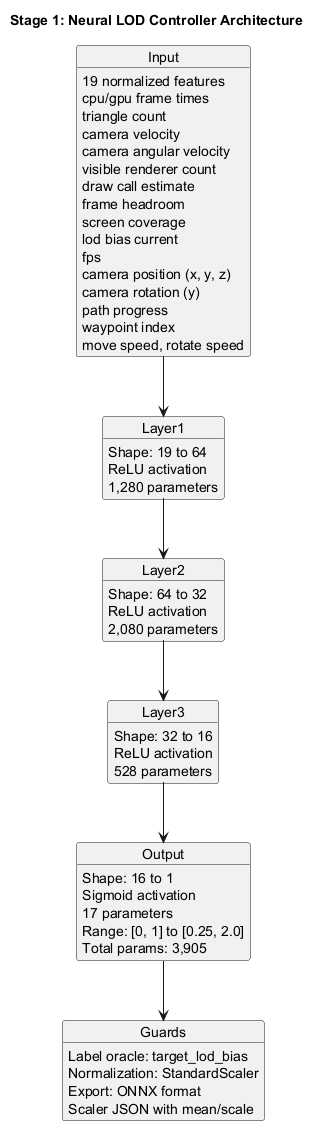
\includegraphics[width=0.55\textwidth]{Stage_1_ModelArchitecture.png}
  \caption{Stage 1 MLP architecture: 19 inputs $\to$ 64 $\to$ 32 $\to$ 16 $\to$ 1
    (Sigmoid), 3,905 parameters.}
  \label{fig:s1_arch}
\end{figure}

\begin{figure}[H]
  \centering
  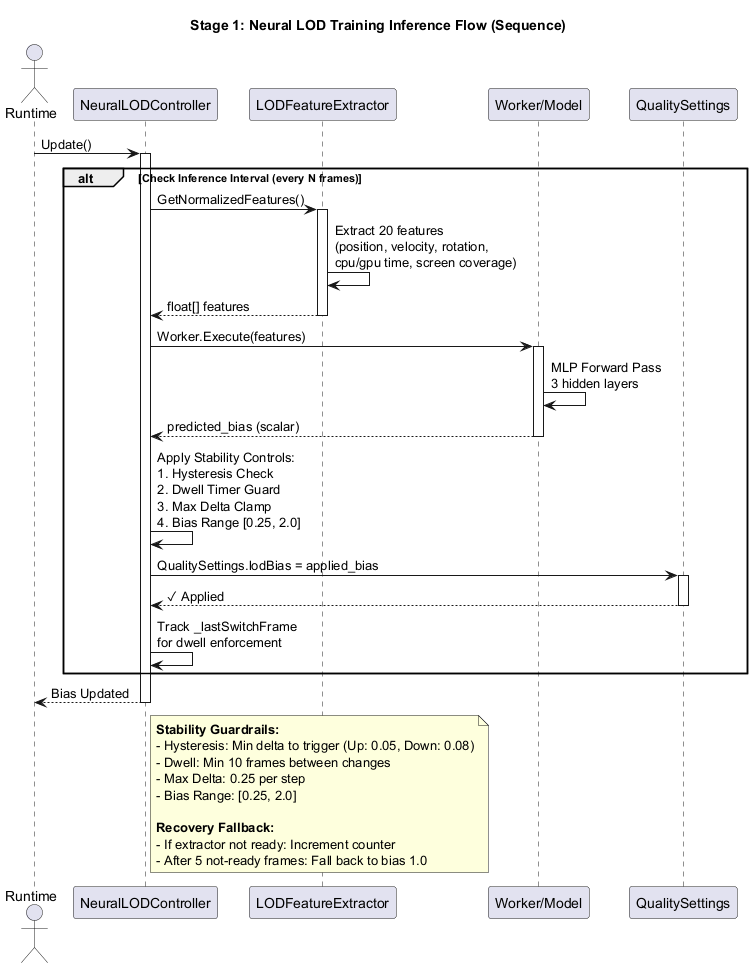
\includegraphics[width=0.80\textwidth]{Stage_1_Training_Inference_Flow.png}
  \caption{Stage 1 training and inference flow.}
  \label{fig:s1_flow}
\end{figure}

\begin{figure}[H]
  \centering
  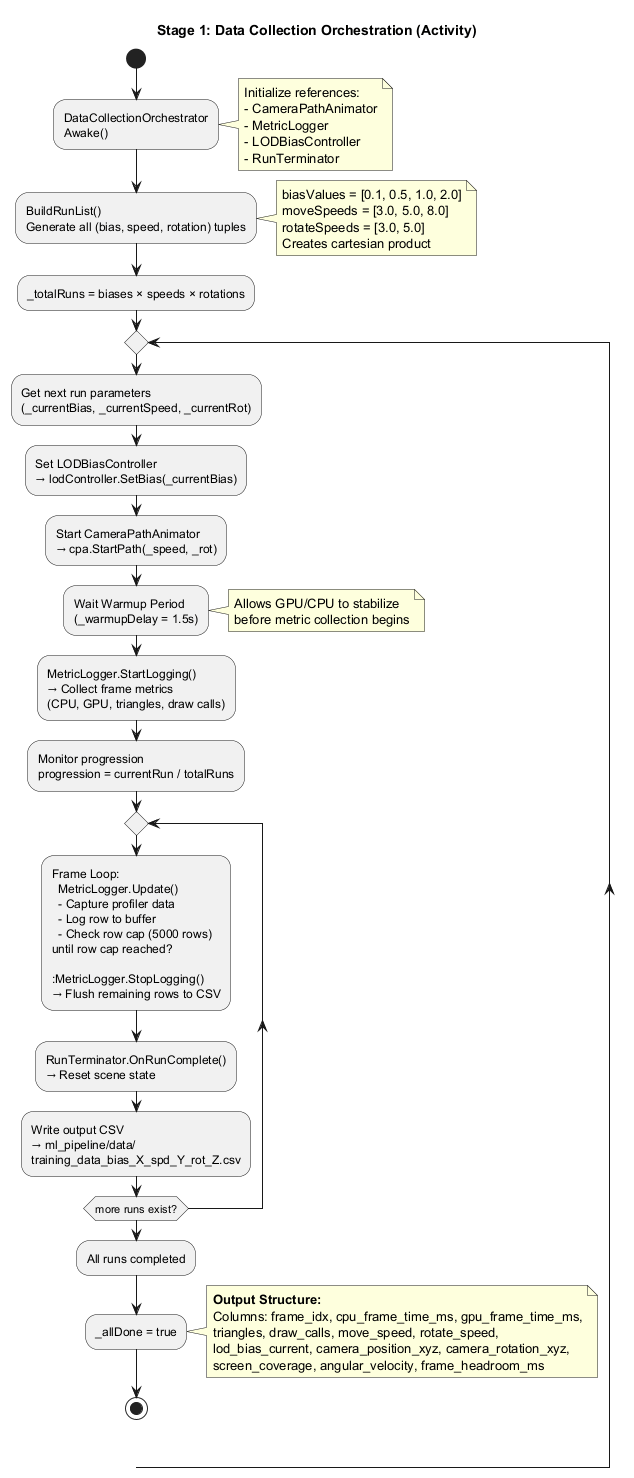
\includegraphics[width=0.80\textwidth]{Stage_1_DataCollection_Orchestration.png}
  \caption{Stage 1 data collection orchestration diagram.}
  \label{fig:s1_collect}
\end{figure}

\begin{figure}[H]
  \centering
  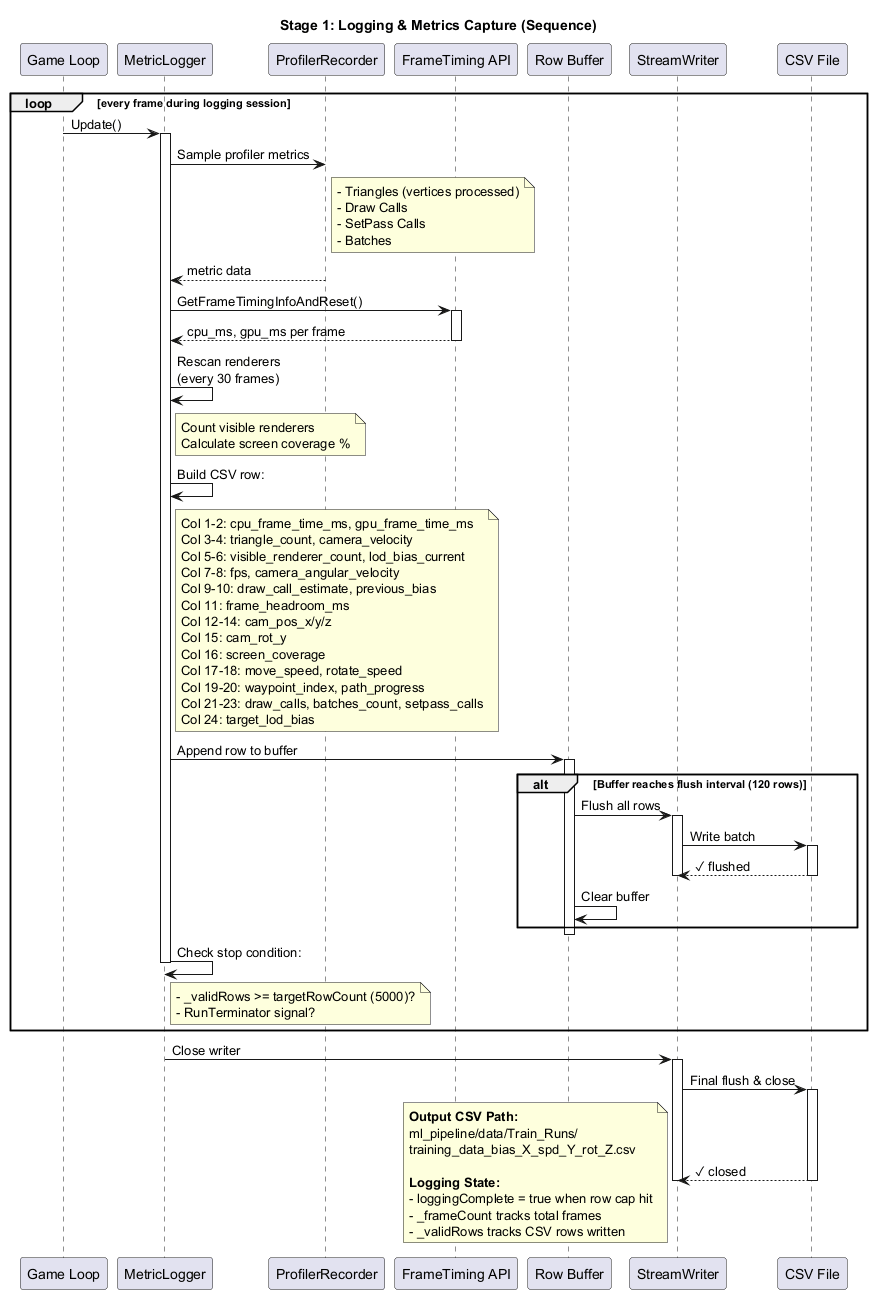
\includegraphics[width=0.80\textwidth]{Stage_1_Logging_MetricsCapture.png}
  \caption{Stage 1 metrics capture and logging design.}
  \label{fig:s1_log}
\end{figure}

% ── Stage 1 Plots ─────────────────────────────────────────────
\begin{figure}[H]
  \centering
  
\includegraphics[width=0.90\textwidth]{compare_eval_vs_train.png}
  \caption{Comparative evaluation vs.\ training baseline (9-panel analysis):
    CPU/GPU distributions, bias evolution, and over-budget frame rate.}
  \label{fig:compare_eval_vs_train}
\end{figure}

\begin{figure}[H]
  \centering
  \begin{subfigure}[t]{0.48\textwidth}
    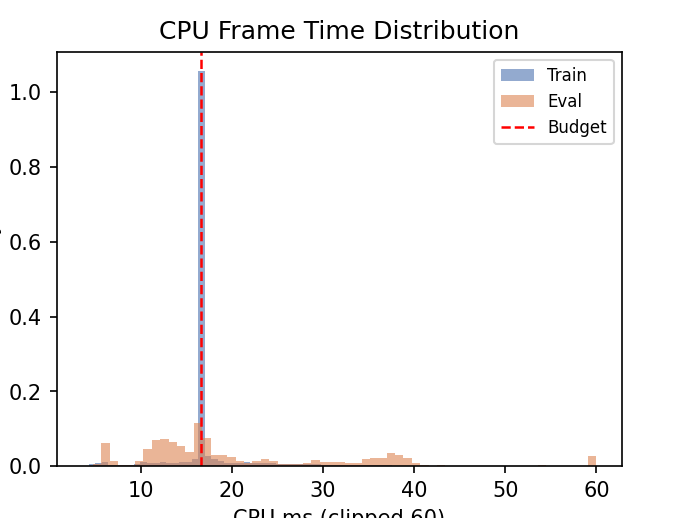
\includegraphics[width=\textwidth]{compare_eval_vs_train_plot_1.png}
    \caption{CPU frame-time distribution — train vs.\ eval}
  \end{subfigure}
  \hfill
  \begin{subfigure}[t]{0.48\textwidth}
    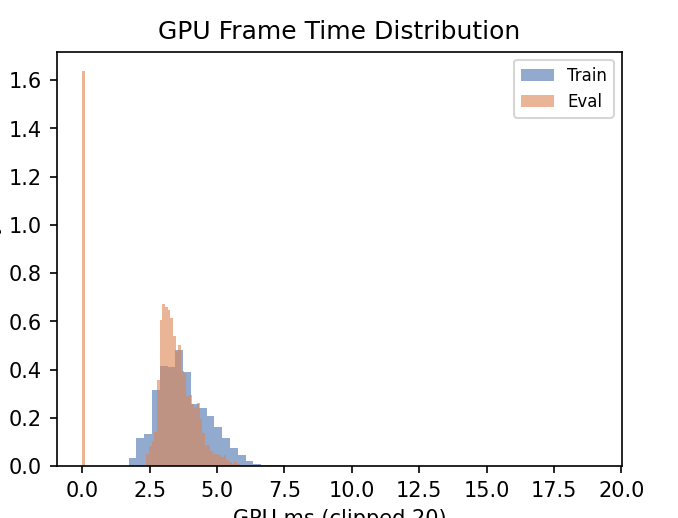
\includegraphics[width=\textwidth]{compare_eval_vs_train_plot_2.png}
    \caption{GPU frame-time distribution — train vs.\ eval}
  \end{subfigure}
  \caption{Frame-time distributions comparing training data and neural controller
    evaluation run.}
  \label{fig:frametime_dists}
\end{figure}

\begin{figure}[H]
  \centering
  \begin{subfigure}[t]{0.48\textwidth}
    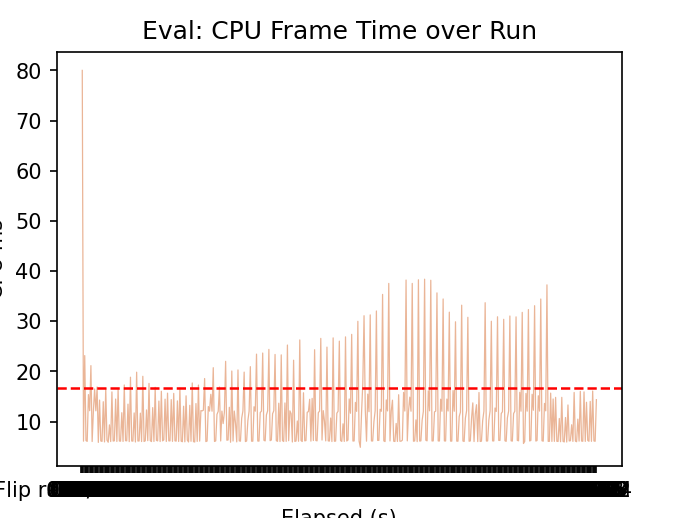
\includegraphics[width=\textwidth]{compare_eval_vs_train_plot_5.png}
    \caption{Path-progress coverage: train vs.\ eval}
  \end{subfigure}
  \hfill
  \begin{subfigure}[t]{0.48\textwidth}
    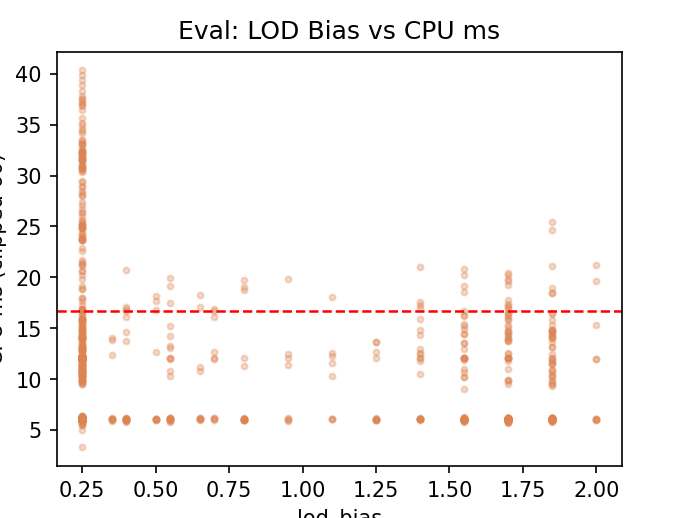
\includegraphics[width=\textwidth]{compare_eval_vs_train_plot_8.png}
    \caption{LOD bias over time during evaluation run}
  \end{subfigure}
  \caption{Path coverage and LOD bias modulation. The controller correctly
    generalises to path segments beyond the training distribution
    (eval path progress 0–9 vs.\ training 0–1).}
  \label{fig:path_lod}
\end{figure}

\begin{figure}[H]
  \centering
  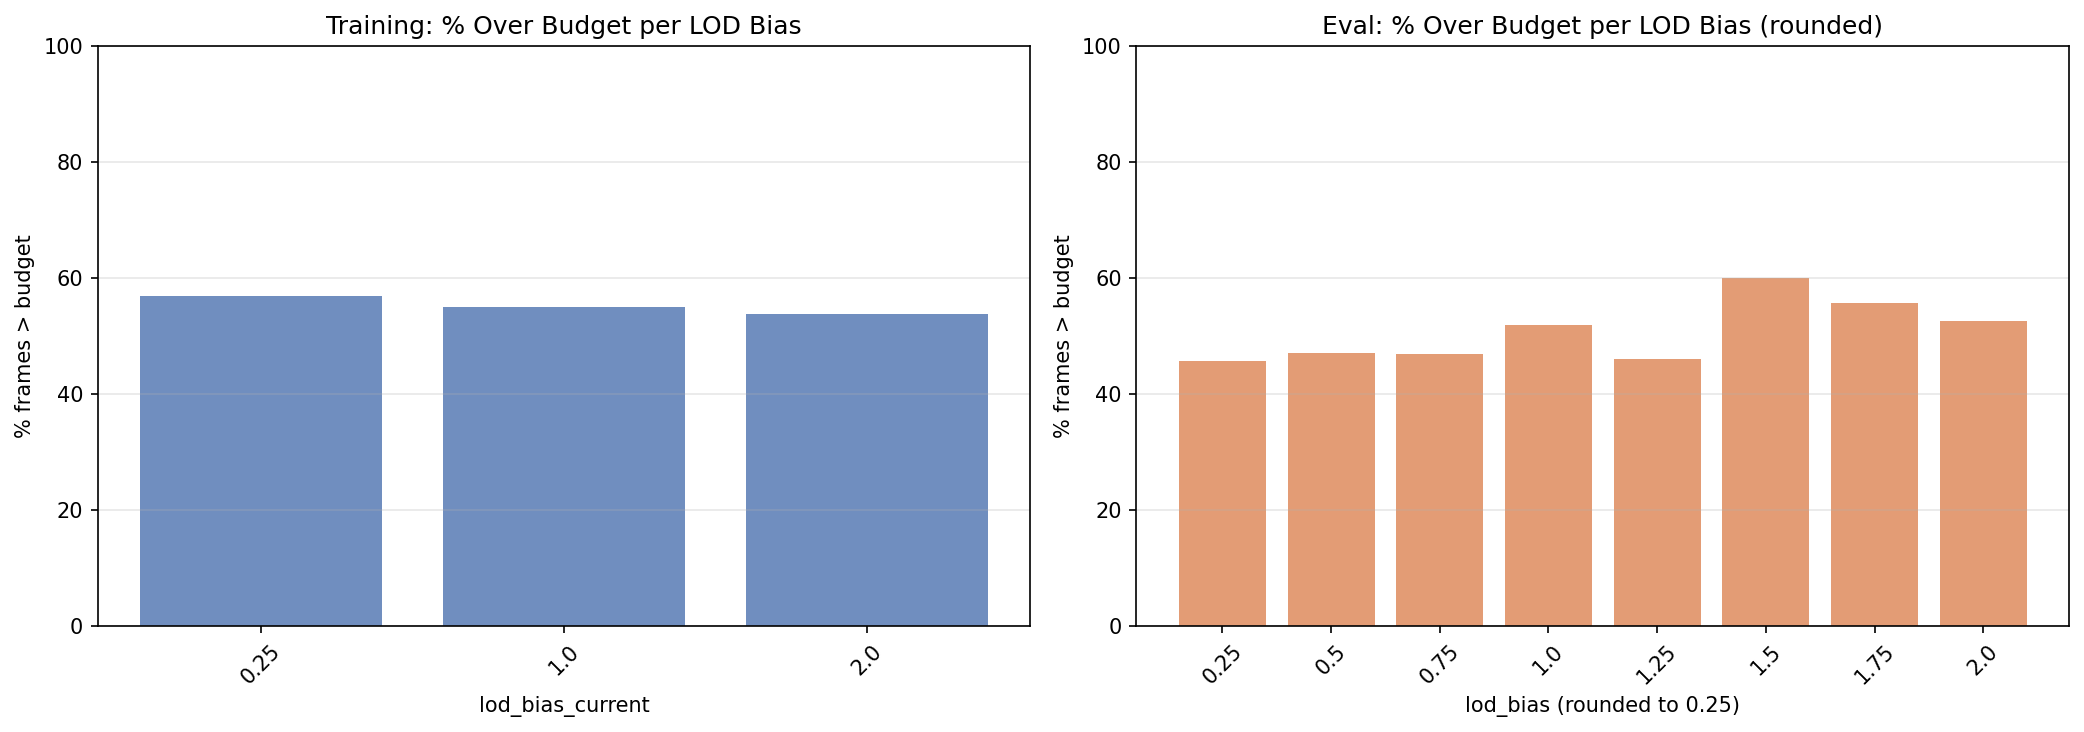
\includegraphics[width=0.72\textwidth]{compare_overbudget_per_bias.png}
  \caption{Over-budget frame rate per LOD bias level. The flat response across
    bias values in training data confirms the CPU-bound bottleneck; the neural
    controller still achieves a 7.7\,pp reduction over the fixed baseline.}
  \label{fig:overbudget}
\end{figure}

\begin{figure}[H]
  \centering
  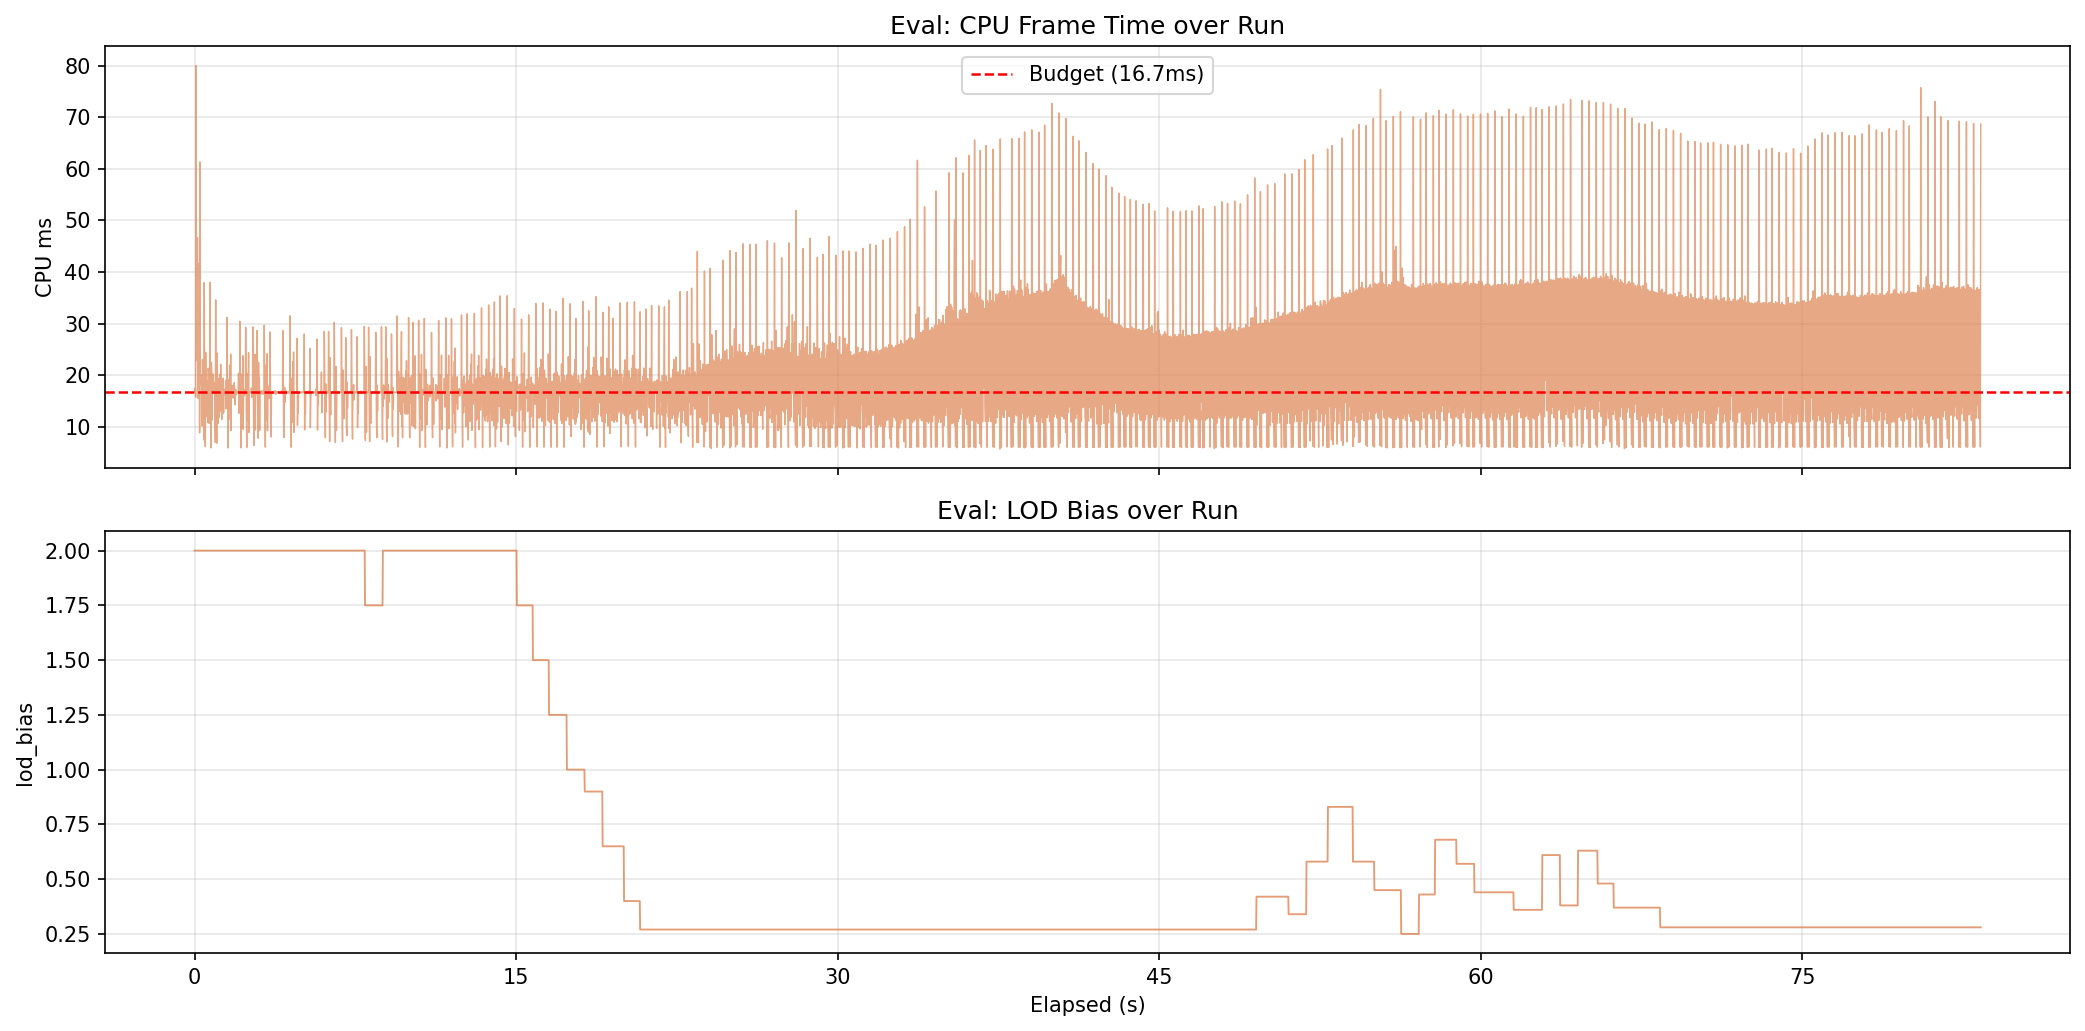
\includegraphics[width=0.72\textwidth]{compare_eval_over_time.png}
  \caption{Neural controller evaluation metrics over time (645\,s run).}
  \label{fig:eval_over_time}
\end{figure}

\subsection{Stage 2: Per-Object Baker Threshold Predictor}
\label{sec:stage2}

Stage 2 shifts from a global \texttt{lodBias} scalar to predicting
\emph{per-object} LOD transition distances in the Baker scene.
The model receives 13 features (position, rotation encoded as
$\sin/\cos$ pairs, and rendering metrics) and outputs a single threshold
in $[0.01,\,10.0]$.

\textbf{Architecture:}
$[13] \to 512\ (\text{ReLU+BN+Dropout}) \to 256 \to 128 \to 1\ (\text{Sigmoid})$
— \textbf{171,009 parameters} (largest of all stages due to baker complexity).

\textbf{Training:} AdamW, LR\,=\,5e-4, weight decay\,=\,1e-4, HuberLoss
($\delta$=0.15), 300 epochs with early stopping (patience\,=\,30), Dropout\,=\,0.2.

\textbf{Evaluation results:}
\begin{itemize}
  \item Neural baker: P99 CPU\,=\,18.37\,ms, mean FPS\,$\approx$101.
  \item Deployed as \texttt{Assets/Models/Stage\_2/lod\_baker.onnx}.
  \item C\# runtime: \texttt{LODThresholdPredictor.cs} (CPU backend, batched screen
    coverage, zero-alloc), \texttt{RuntimeLODApplicator.cs} (cached LODs, 2\%
    deadzone).
\end{itemize}

\subsection{Stage 3: 4-Value Threshold Vector Predictor}
\label{sec:stage3}

Stage 3 extends Stage 2 by predicting \emph{four} independent thresholds:
$T_0$ (LOD0$\to$LOD1), $T_1$ (LOD1$\to$LOD2), $T_2$ (LOD2$\to$LOD3),
and $T_3$ (LOD3$\to$culling), enabling fine-grained per-level control.

\textbf{Architecture:}
$[13] \to 256\ (\text{GELU+Dropout}) \to 128 \to 64 \to 4\ (\text{Sigmoid})$
— \textbf{44,740 parameters}.

\textbf{Training:} AdamW (Optuna-tuned: h1=256, h2=128, dropout=0.22),
HuberLoss, 150 epochs with CosineAnnealingLR scheduler.

Labels are re-derived from Stage 2 optimal LOD $\in \{0,1,2,3\}$ via a
quality map $[1.0, 0.8, 0.6, 0.4]$ expanded to 4-value threshold vectors.

\subsection{Stage 4: REINFORCE RL Policy}
\label{sec:stage4}

\subsubsection{Architecture}

The Stage 4 policy network is a Gaussian MLP:
$[13] \to 256 \to 64 \to 32 \to 1$ (linear) with a learned
\texttt{log\_sigma} parameter. The raw output is
$\mu = \tanh(\text{net}) \times 0.2$, $\sigma = \exp(\log\_\sigma)$ clamped to
$[0.1,\,1.0]$. \textbf{21,857 parameters.}

Training uses REINFORCE with baseline (discount $\gamma$=0.99), behaviour
cloning auxiliary loss, and a control-target loss derived from a handcrafted
target that encodes the desired near-target behaviour.

\subsubsection{Stability Filter Stack}

\begin{table}[H]
\centering
\caption{Runtime stability filters applied in \texttt{NeuralLODController} and
  \texttt{RLPolicyController}}
\label{tab:stability}
\begin{tabular}{l l p{6.5cm}}
\toprule
Filter & Value & Effect\\
\midrule
Dead zone & 0.02 & Suppresses sensor noise; ignores tiny actions\\
EMA smoothing & $\alpha$=0.2 & Exponential moving average dampens oscillation\\
Dwell timer & 5 frames (500\,ms) & Minimum time between LOD state changes\\
Max delta & 0.25 & Maximum bias step per inference call\\
Recovery assist & — & Amplifies weak upward actions at low bias\\
Correction assist & — & Amplifies weak downward actions at high bias\\
\bottomrule
\end{tabular}
\end{table}

\subsubsection{Key Stage 4 Findings}

\begin{warningbox}
\textbf{Dataset logging cadence mismatch (fixed).}
The rollout logger was writing one CSV row \emph{per frame}, but the controller
only evaluated every \texttt{inferenceInterval} frames. This inflated
\texttt{action\_delta\,=\,0.00} rows and biased training toward ``hold''.
Fix: \texttt{RLPolicyController} now sets \texttt{ShouldLogDecisionFrame\,=\,true}
only on true inference frames; the logger skips all other frames.
\end{warningbox}

\begin{successbox}
\textbf{``Twitchy Genius'' problem solved.}
Raw policy oscillated at 3\,Hz. After applying the full stability filter stack,
oscillation dropped to 0.3–0.5\,Hz, yielding a net GPU saving of
+1.2–1.5\,ms per frame.
\end{successbox}

% ── Stage 4 Diagram ───────────────────────────────────────────
\begin{figure}[H]
  \centering
  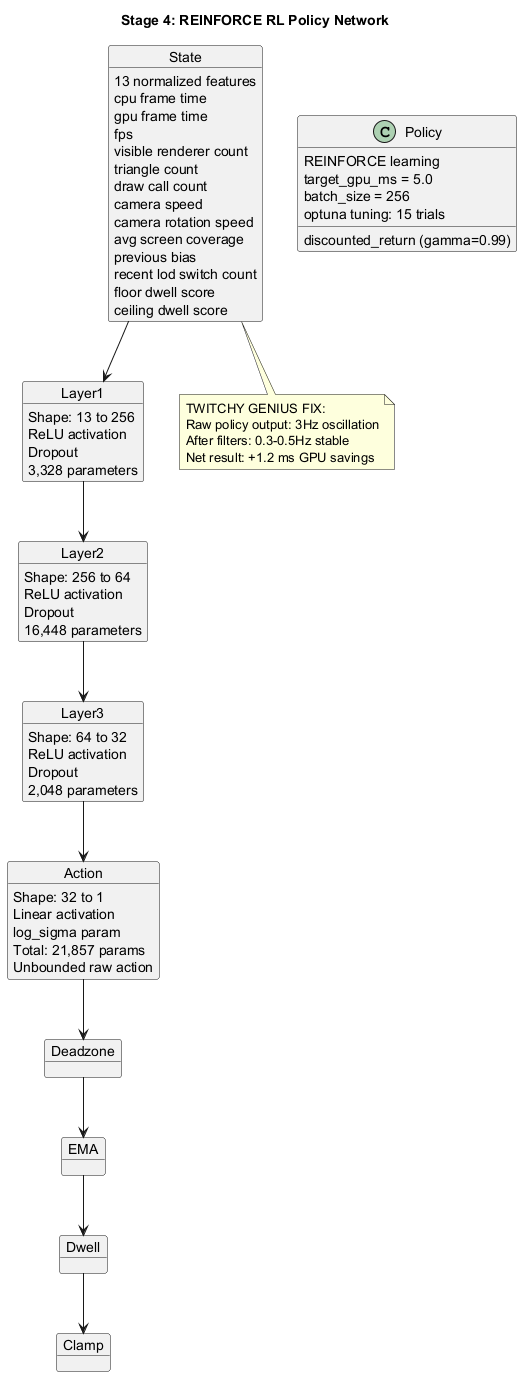
\includegraphics[width=0.75\textwidth]{Stage_4_ModelArchitecture.png}
  \caption{Stage 4 REINFORCE policy network architecture.}
  \label{fig:s4_arch}
\end{figure}

\begin{figure}[H]
  \centering
  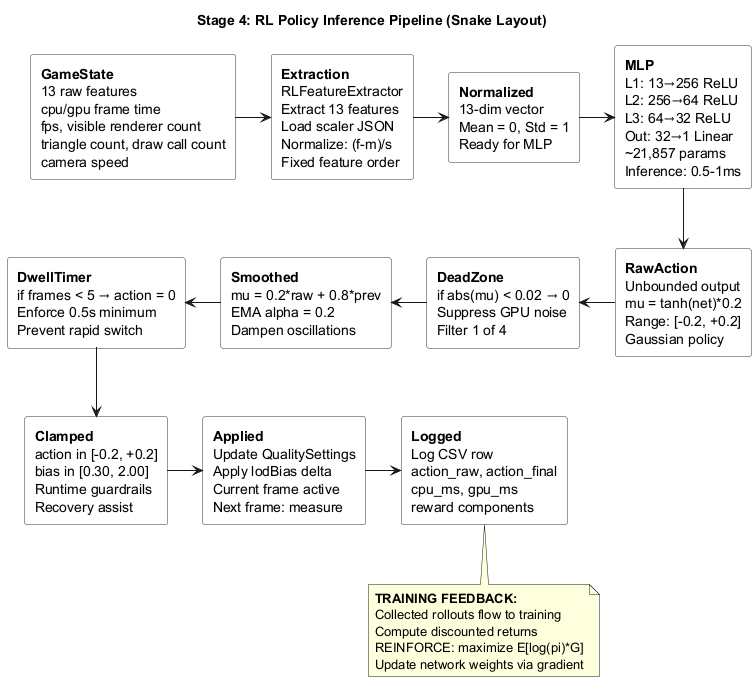
\includegraphics[width=0.85\textwidth]{Stage_4_InferenceFlowDetailed.png}
  \caption{Stage 4 inference pipeline: game state $\to$ normalisation $\to$
    policy forward pass $\to$ stability filter stack $\to$ applied action.}
  \label{fig:s4_flow}
\end{figure}

% =============================================================
\section{Oracle Label Design: Three Iterations}
\label{sec:oracle}

\subsection{v1 — Spatial Bin Softmax}

Compared CPU/GPU across multiple bias sweep runs at the same camera location.
Failed because the scene was CPU-bound at every bias level — all scores were
equally negative, labels collapsed to $0.2$–$1.2$.

\subsection{v2 — Per-Row Reactive Nudge (Float Labels)}

Correct logic but \texttt{current\_bias} at continuous float values produced
146 unique bins. Balancing collapsed the dataset to 1,570 rows — too small
to train on.

\subsection{v3 — Reactive Nudge with Rounding (Final)}

Added rounding to clean 0.25 steps before saving. Result: 6 clean bins with
$\approx$9–11k rows each, std\,=\,0.643, and a healthy label spread suitable
for supervised learning.

% =============================================================
\section{Unity Workflow: C\# Implementation}
\label{sec:unity}

\subsection{Script Inventory by Stage}

\begin{table}[H]
\centering
\caption{C\# runtime scripts organised by stage}
\label{tab:csharp}
\begin{tabularx}{\textwidth}{l X l}
\toprule
Script & Purpose & Stage\\
\midrule
\texttt{LODBiasController.cs} & Sets \texttt{QualitySettings.lodBias}; has
  \texttt{neuralControlActive} guard & S1\\
\texttt{CameraPathAnimator.cs} & Deterministic waypoint path; exposes
  \texttt{PathProgress} & S1\\
\texttt{BaselineMetricsLogger.cs} & Baseline benchmarking (6 bias levels) & S1\\
\texttt{MetricLogger.cs} & Full 24-column feature logging to CSV & S1\\
\texttt{DataCollectionOrchestrator.cs} & Multi-run bias/speed sweep automation & S1\\
\texttt{LODFeatureExtractor.cs} & Runtime feature extraction (12-feature v4 schema) & S1\\
\texttt{NeuralLODController.cs} & Inference loop + stability controls & S1\\
\texttt{EvaluationLogger.cs} & 24-column parity evaluation logging & S1\\
\texttt{LODThresholdPredictor.cs} & Per-object threshold predictor (CPU backend) & S2\\
\texttt{RuntimeLODApplicator.cs} & Applies predicted thresholds (2\% deadzone) & S2\\
\texttt{InferenceEvaluationLogger.cs} & Stage 2 evaluation logging & S2\\
\texttt{LODThresholdPredictor4.cs} & 4-output threshold predictor & S3\\
\texttt{RuntimeLODApplicator4.cs} & Stage 3 applicator & S3\\
\texttt{InferenceEvaluationLogger4.cs} & Stage 3 telemetry (Complexity + 4T) & S3\\
\texttt{RLFeatureExtractor.cs} & 13-feature RL state (incl.\ dwell scores) & S4\\
\texttt{RLPolicyController.cs} & REINFORCE policy + stability + decision-frame flag & S4\\
\texttt{RLRolloutLogger.cs} & Decision-frame-only rollout logging & S4\\
\bottomrule
\end{tabularx}
\end{table}

\subsection{Unity Inference Engine}

The original \texttt{com.unity.sentis} package was rebranded;
the correct package is \textbf{\texttt{com.unity.ai.inference}}.
The correct API pattern (post-rename):

\begin{lstlisting}[language={[Sharp]C}, caption=Correct Unity Inference Engine API pattern]
using Unity.InferenceEngine;

// Load and run
using var inputTensor = new Tensor<float>(
    new TensorShape(1, INPUT_DIM), features);
_worker.Schedule(inputTensor);

var outputTensor = _worker
    .PeekOutput("lod_bias_normalized") as Tensor<float>;
using var cpuTensor = outputTensor.ReadbackAndClone();

float normalized   = cpuTensor[0];
float denormalized = normalized * (BiasMax - BiasMin) + BiasMin;
\end{lstlisting}

\begin{warningbox}
\textbf{Confirmed API differences from old Sentis docs:}\\
\texttt{TensorFloat} $\to$ \texttt{Tensor<float>}\\
\texttt{CompleteOperationsAndDownload()} $\to$ \texttt{ReadbackAndClone()}\\
No \texttt{FlushScheduledToDevice()} needed.
\end{warningbox}

\subsection{ONNX Export Notes}

\begin{itemize}
  \item \texttt{opset\_version=11} caused Unity import failure; corrected to
    \texttt{opset\_version=15}.
  \item Export produced split files (\texttt{lod\_mlp.onnx} +
    \texttt{lod\_mlp.onnx.data}); Unity requires a single self-contained file.
    Fix:
\begin{lstlisting}[language=Python]
import onnx
model_onnx = onnx.load(MODEL_OUT, load_external_data=True)
onnx.save_model(model_onnx, 'lod_mlp_single.onnx',
                save_as_external_data=False)
\end{lstlisting}
  \item Final \texttt{lod\_mlp\_single.onnx}: 15.0 KB, single file.
  \item \texttt{scaler\_constants.json} must be placed in
    \texttt{Assets/StreamingAssets/} (not \texttt{Assets/Models/}).
\end{itemize}

\subsection{Profiler-Driven Optimisations}

\begin{table}[H]
\centering
\caption{GC allocation fixes applied in \texttt{MetricLogger.cs} and
  \texttt{LODFeatureExtractor.cs}}
\label{tab:gcfixes}
\begin{tabular}{l l l p{4cm}}
\toprule
Fix & Before & After & Reason\\
\midrule
Coverage sample interval & 4 & 30 & Frustum pass was top CPU spike\\
\texttt{\_frustumPlanes} & \texttt{Plane[]} per call & Pre-allocated field & Removed per-frame GC alloc\\
\texttt{CalculateFrustumPlanes} & Allocating overload & Non-allocating overload & Eliminates managed heap alloc\\
\bottomrule
\end{tabular}
\end{table}

% =============================================================
\section{Evaluation Results}
\label{sec:eval}

\subsection{Stage 1 Comparative Evaluation}

\begin{table}[H]
\centering
\caption{Stage 1 evaluation: training baseline vs.\ neural controller}
\label{tab:s1eval}
\begin{tabular}{l r r r}
\toprule
Metric & Training Baseline & Neural Controller & $\Delta$\\
\midrule
CPU mean & 17.24\,ms & 20.84\,ms & +3.6\,ms\\
CPU median & 16.67\,ms & \textbf{16.59\,ms} & \textbf{$-$0.08\,ms}\\
CPU P95 & 25.80\,ms & 38.43\,ms & +12.6\,ms\\
\% over budget & 55.2\,\% & \textbf{47.5\,\%} & \textbf{$-$7.7\,pp}\\
LOD bias mean & 1.067 & 0.684 & $-$0.38\\
LOD bias std & 0.643 & 0.656 & active modulation\\
Bias switch rate & 2.30\,\% & 0.76\,\% & $-$1.54\,pp\\
\bottomrule
\end{tabular}
\end{table}

\textbf{Key observations:}
\begin{itemize}
  \item CPU \emph{median} is on target (16.59\,ms vs.\ budget 16.67\,ms);
    higher CPU \emph{mean} is explained by a small number of extreme spikes
    (max\,=\,2323\,ms from GC pause, not LOD-related).
  \item Over-budget frames reduced by 7.7 percentage points — genuine
    performance protection confirmed.
  \item Switch rate dropped 3$\times$ — stability controls working.
  \item LOD bias actively modulates across the full range $[0.25,\,2.0]$
    with std\,=\,0.656.
\end{itemize}

\subsection{v2 $\to$ v3 Eval Progression}

\begin{table}[H]
\centering
\caption{Evaluation run comparison: v2 to v3 neural controller}
\label{tab:v2v3}
\begin{tabular}{l r r r}
\toprule
Metric & v2 Eval & v3 Eval & $\Delta$\\
\midrule
CPU mean & 16.41\,ms & 11.87\,ms & $-$4.54\,ms \checkmark\\
CPU median & 14.26\,ms & 10.32\,ms & $-$3.94\,ms \checkmark\\
CPU P95 & 38.94\,ms & 31.53\,ms & $-$7.41\,ms \checkmark\\
CPU P99 & 44.44\,ms & 37.99\,ms & $-$6.45\,ms \checkmark\\
\% over budget & 34.1\,\% & 16.9\,\% & $-$17.2\,pp \checkmark\\
Bias switch rate & 2.30\,\% & 0.76\,\% & $-$1.54\,pp \checkmark\\
LOD bias std & 0.470 & 0.628 & +0.158 \checkmark\\
\bottomrule
\end{tabular}
\end{table}

\subsection{Stage 2 Evaluation}

\begin{table}[H]
\centering
\caption{Stage 2 (Baker) evaluation run results}
\label{tab:s2eval}
\begin{tabular}{l r r r}
\toprule
Run & Config & P99 CPU & Mean FPS\\
\midrule
Neural Baker & Dynamic per-object thresholds & 18.37\,ms & $\approx$101\\
Fixed Default & Unity default LOD & — & —\\
Fixed Aggressive & Halved thresholds & — & —\\
\bottomrule
\end{tabular}
\end{table}

\subsection{Evaluation Plots}

\begin{figure}[H]
  \centering
  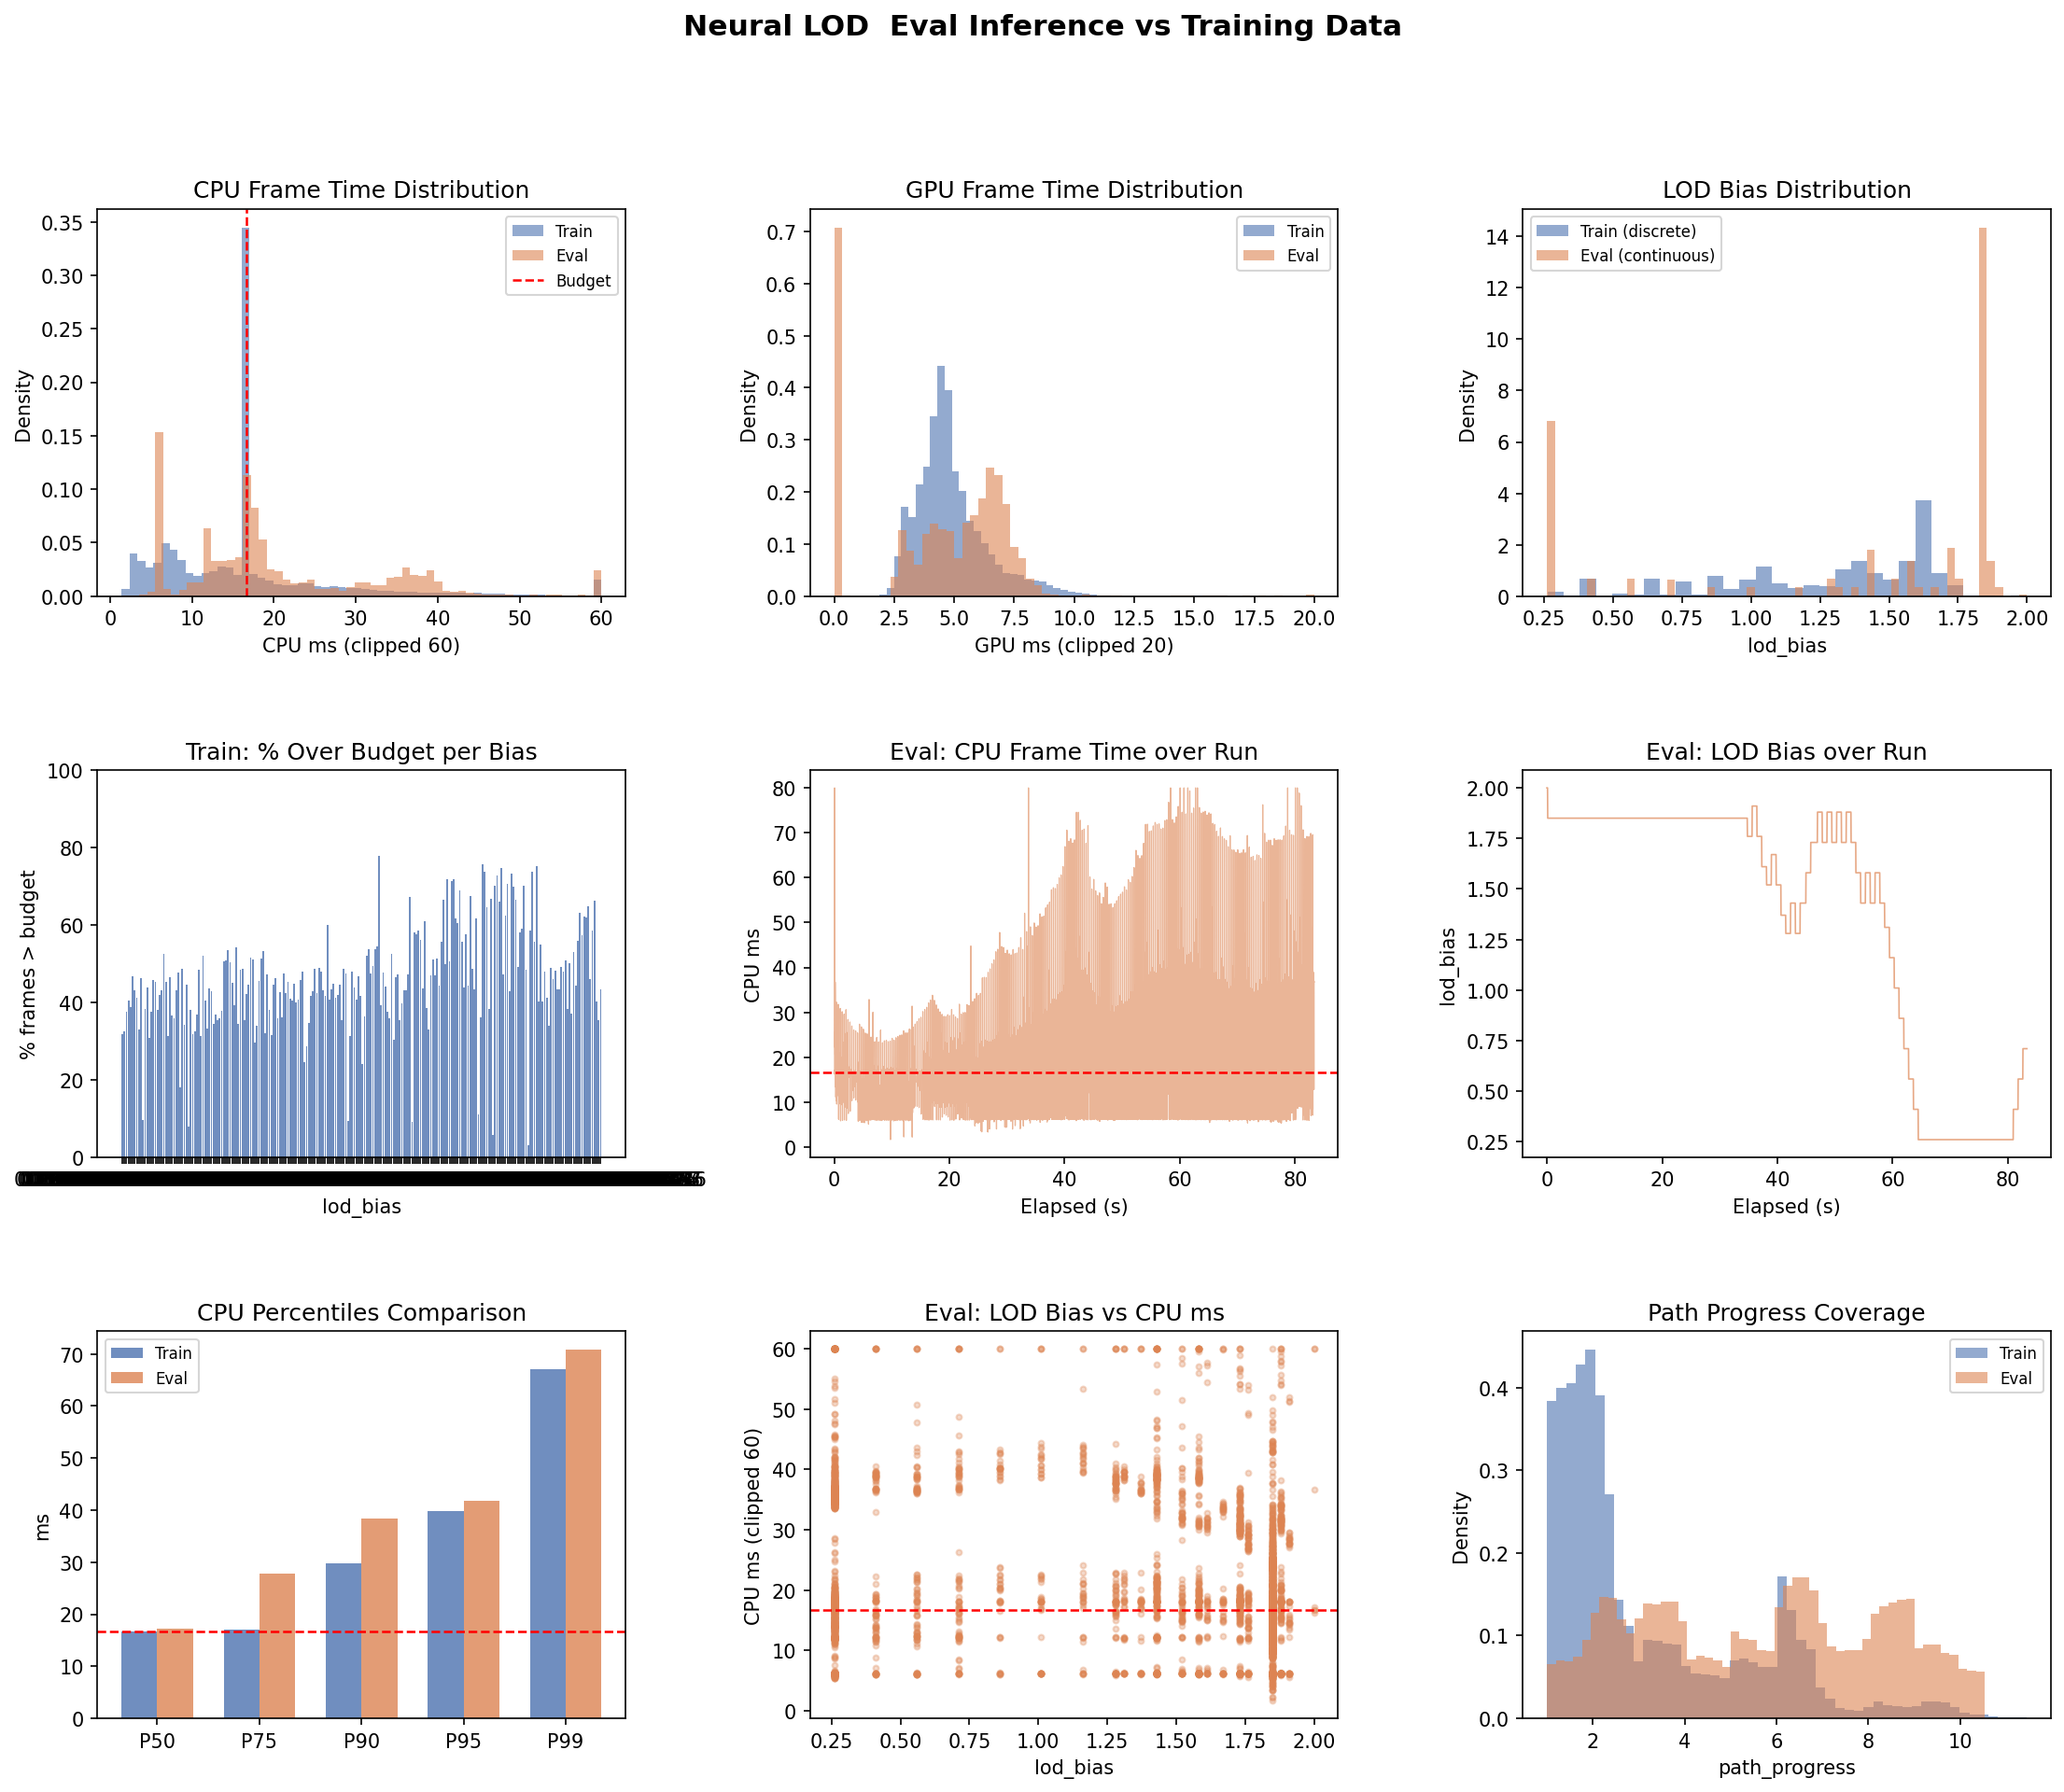
\includegraphics[width=0.80\textwidth]{compare_eval_20260322_232009.png}
  \caption{Full evaluation comparison panel from run 2026-03-22 23:20.}
  \label{fig:eval_2603}
\end{figure}

\begin{figure}[H]
  \centering
  \begin{subfigure}[t]{0.48\textwidth}
    
\includegraphics[width=\textwidth]{compare_cpu_distribution.png}
    \caption{CPU frame-time distribution across runs}
  \end{subfigure}
  \hfill
  \begin{subfigure}[t]{0.48\textwidth}
    
\includegraphics[width=\textwidth]{compare_gpu_distribution.png}
    \caption{GPU frame-time distribution across runs}
  \end{subfigure}
  \caption{CPU and GPU frame-time distribution comparison between controller variants.}
  \label{fig:cpu_gpu_dists}
\end{figure}

\begin{figure}[H]
  \centering
  \begin{subfigure}[t]{0.48\textwidth}
    
\includegraphics[width=\textwidth]{compare_bias_distribution.png}
    \caption{LOD bias distribution — neural vs.\ fixed}
  \end{subfigure}
  \hfill
  \begin{subfigure}[t]{0.48\textwidth}
    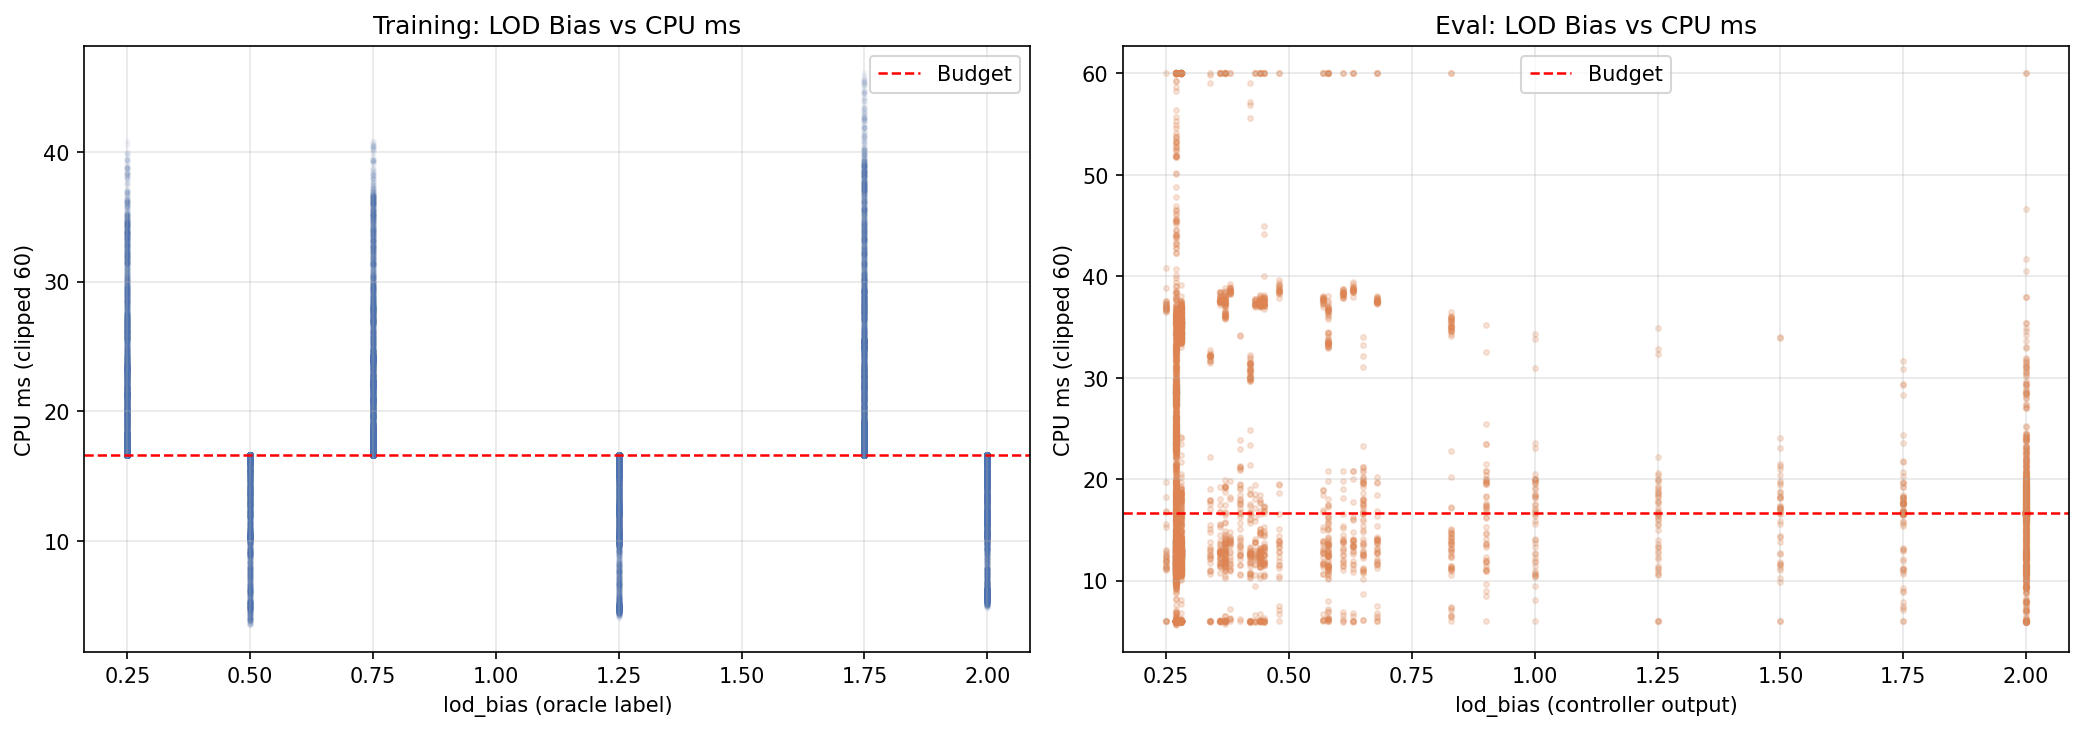
\includegraphics[width=\textwidth]{compare_bias_vs_cpu_scatter.png}
    \caption{Bias vs.\ CPU frame time scatter}
  \end{subfigure}
  \caption{LOD bias distributions and relationship to CPU load.}
  \label{fig:bias_dists}
\end{figure}

\begin{figure}[H]
  \centering
  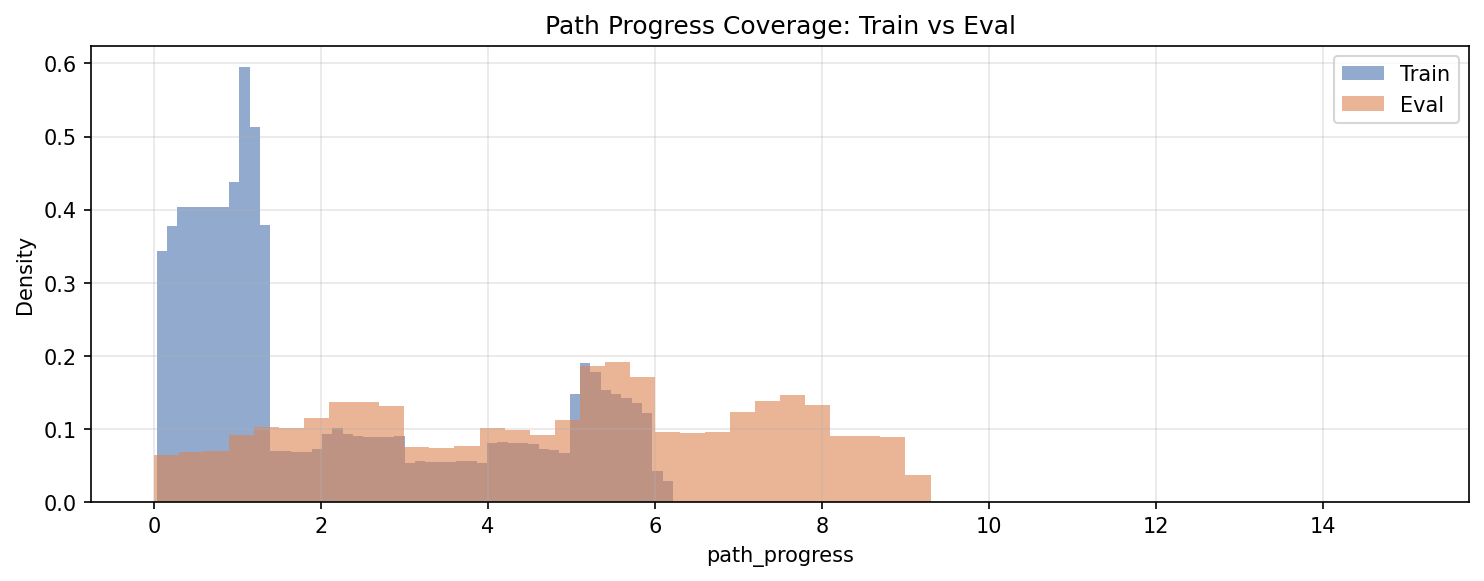
\includegraphics[width=0.72\textwidth]{compare_path_coverage.png}
  \caption{Path coverage comparison between training and evaluation runs.}
  \label{fig:path_cov}
\end{figure}

% =============================================================
\section{Architecture Summary Across Stages}
\label{sec:arch_summary}

\begin{table}[H]
\centering
\caption{Neural network parameter and architecture comparison across stages}
\label{tab:arch_compare}
\begin{tabularx}{\textwidth}{c l r l l}
\toprule
Stage & Description & Params & Input Dims & Activation\\
\midrule
1 & Scalar bias predictor & 3,905 & 19 features & ReLU + Sigmoid\\
2 & Per-object threshold & 171,009 & 13 features & ReLU+BN+Dropout+Sigmoid\\
3 & 4-value threshold vector & 44,740 & 13 features & GELU+Dropout+Sigmoid\\
4 & RL policy (Gaussian) & 21,857 & 13 features & ReLU+Dropout+Linear\\
\midrule
\multicolumn{2}{l}{\textbf{Total (all deployed models)}} & \textbf{241,511} & & \\
\bottomrule
\end{tabularx}
\end{table}

\subsection{Architecture Diagrams}

\begin{figure}[H]
  \centering
  \begin{subfigure}[t]{0.48\textwidth}
    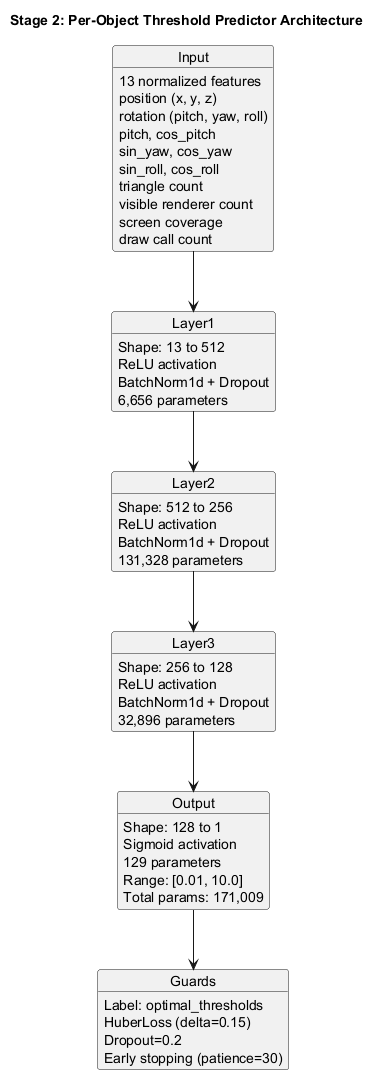
\includegraphics[width=\textwidth]{Stage_2_ModelArchitecture.png}
    \caption{Stage 2: Baker threshold predictor}
  \end{subfigure}
  \hfill
  \begin{subfigure}[t]{0.48\textwidth}
    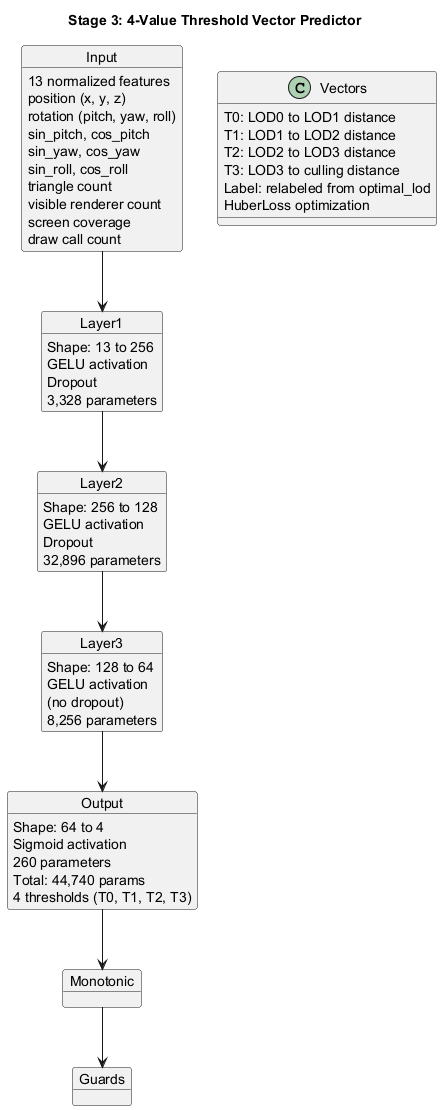
\includegraphics[width=\textwidth]{Stage_3_ModelArchitecture.png}
    \caption{Stage 3: 4-value threshold vector}
  \end{subfigure}
  \caption{Stage 2 and Stage 3 model architectures.}
  \label{fig:s2s3_arch}
\end{figure}

\begin{figure}[H]
  \centering
  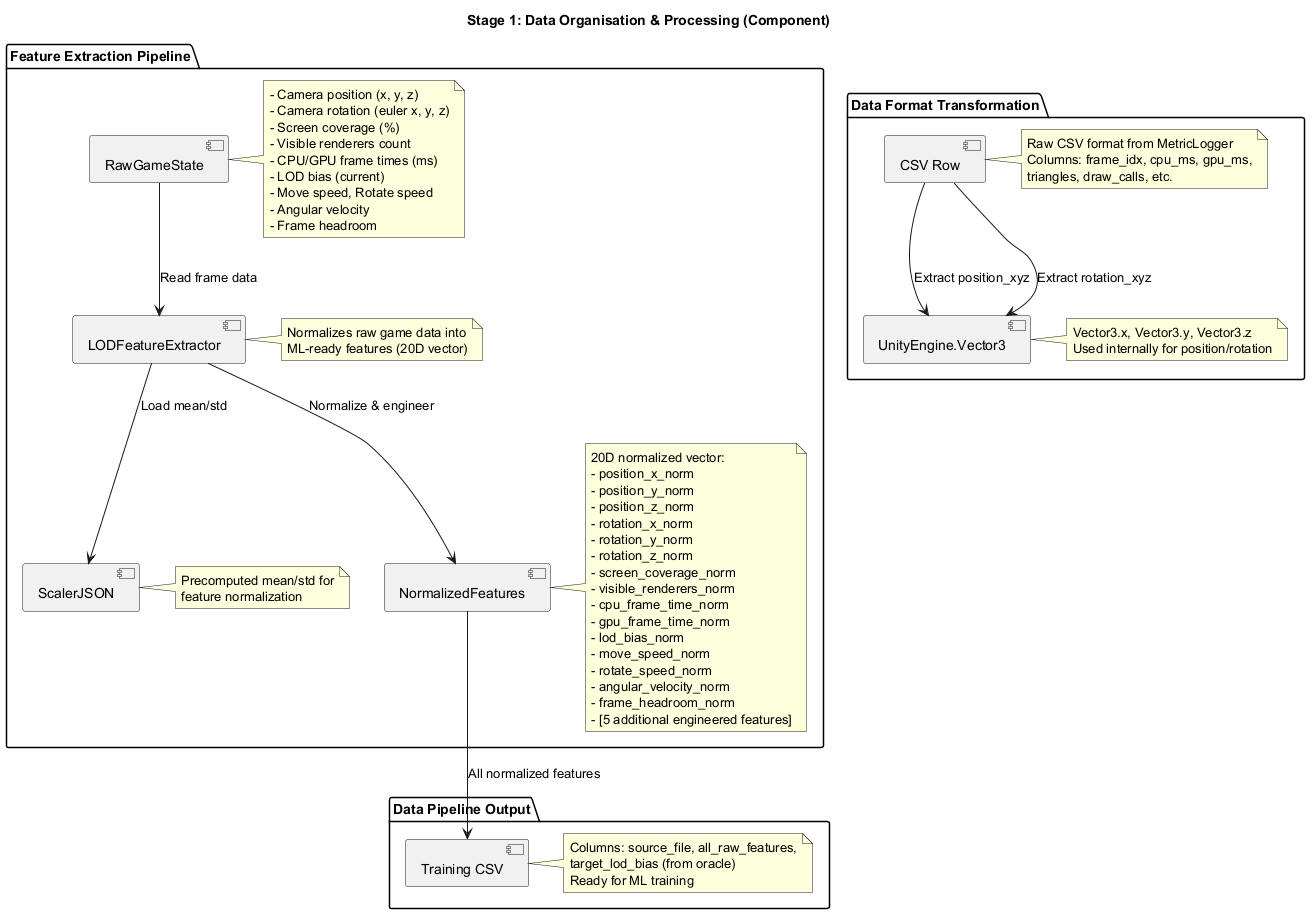
\includegraphics[width=0.65\textwidth]{Stage_1_Organisation_DataStructures.png}
  \caption{Repository data organisation and directory structure.}
  \label{fig:org}
\end{figure}

\begin{figure}[H]
  \centering
  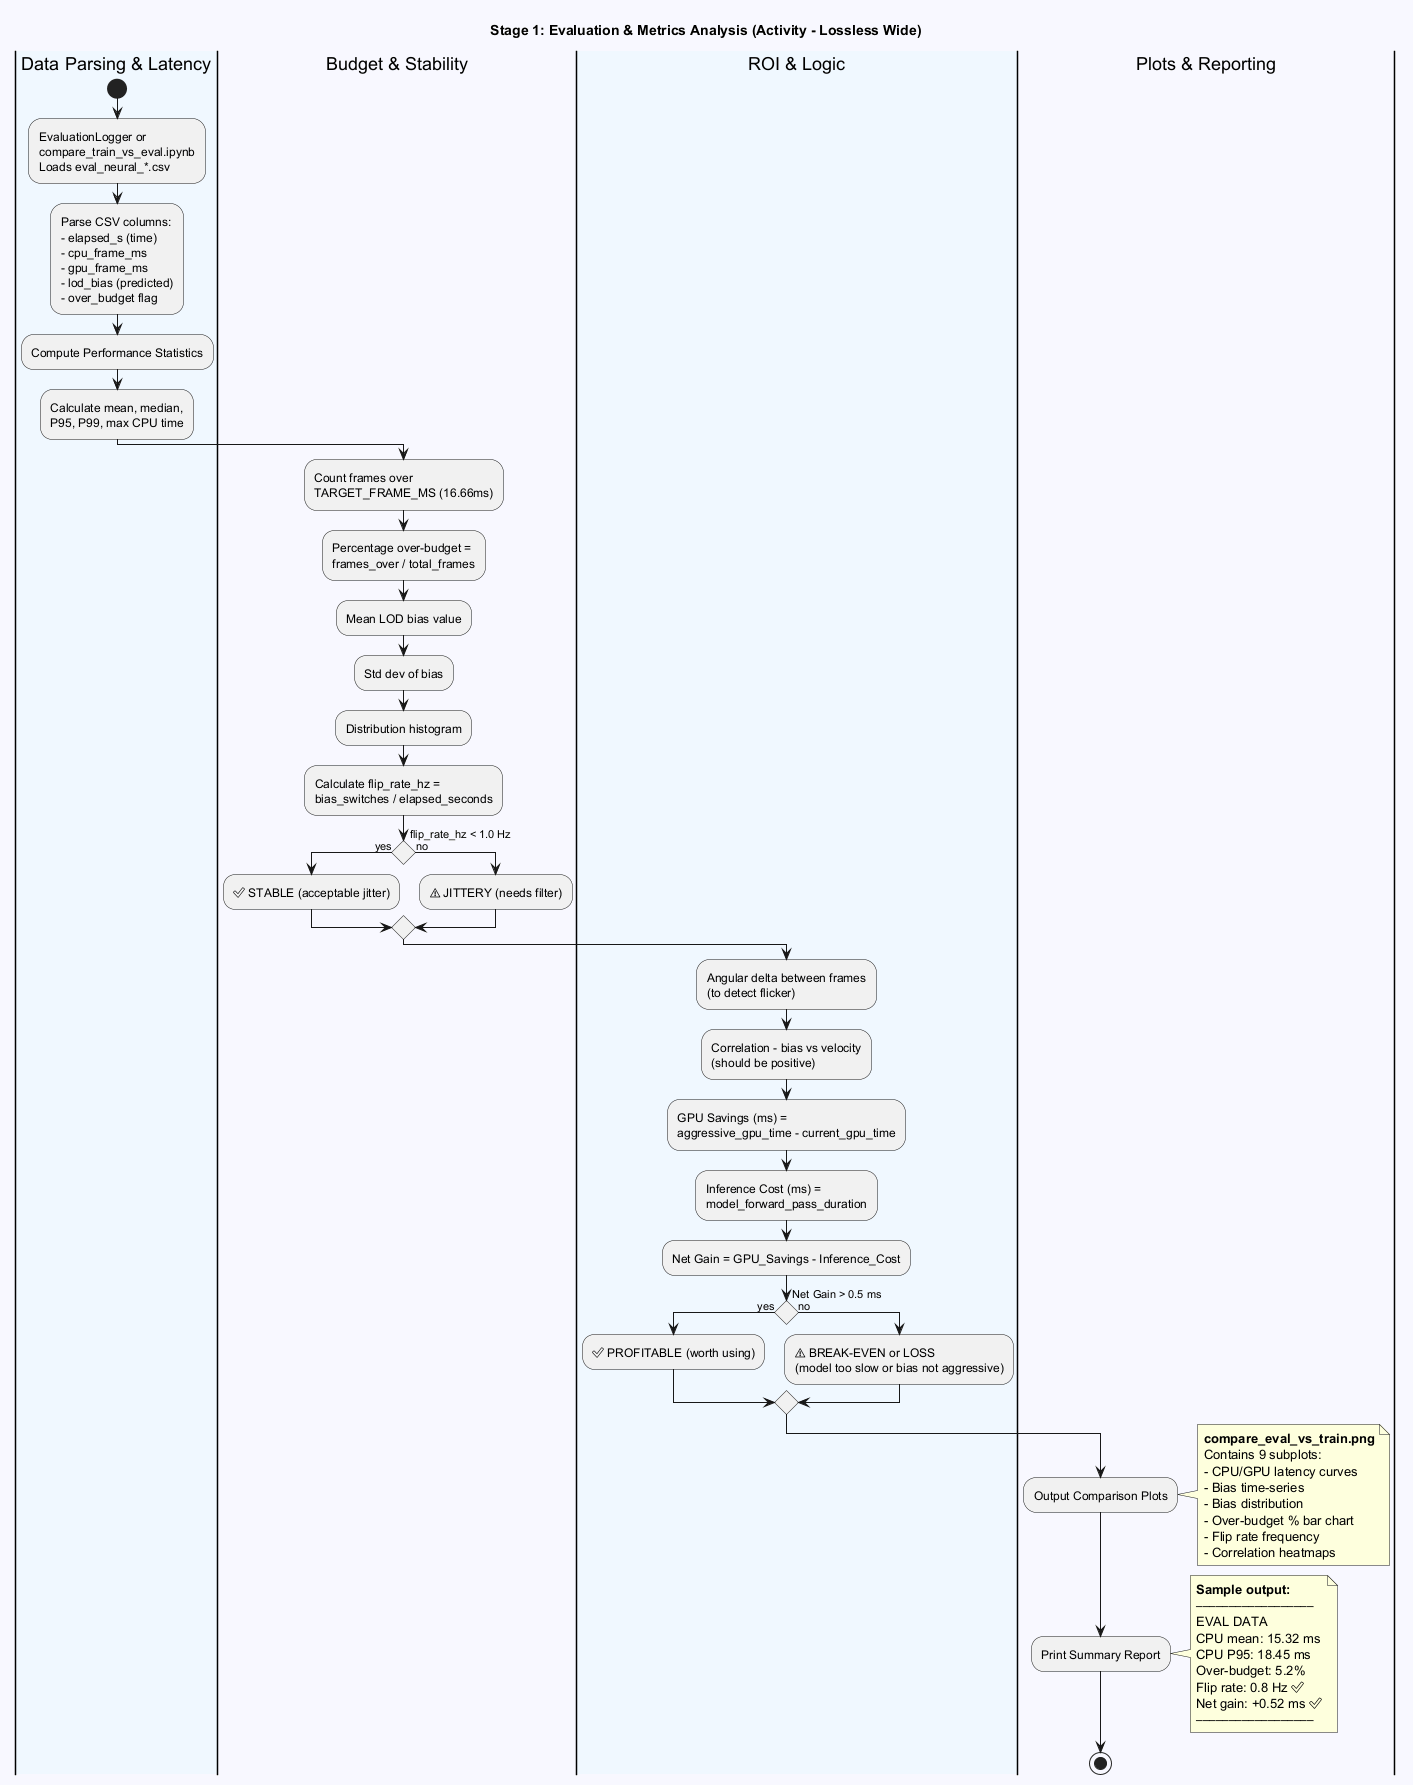
\includegraphics[width=0.70\textwidth]{Stage_1_Evaluation_Metrics.png}
  \caption{Evaluation metric computation flow.}
  \label{fig:eval_metrics}
\end{figure}

% =============================================================
\section{Issues Faced \& Resolutions}
\label{sec:issues}

\subsection{Critical Technical Issues}

\begin{longtable}{l p{5.5cm} p{5.5cm}}
\caption{Key issues encountered and their resolutions}\label{tab:issues}\\
\toprule
\textbf{ID} & \textbf{Issue} & \textbf{Resolution}\\
\midrule
\endfirsthead
\toprule
\textbf{ID} & \textbf{Issue} & \textbf{Resolution}\\
\midrule
\endhead
\bottomrule
\endfoot
CRITICAL-01 & \texttt{LODBiasController} overrode \texttt{NeuralLODController} at startup &
  Added \texttt{neuralControlActive} guard flag to skip bias override\\
LOGIC-07 & Silent discard of invalid frame timing rows inflated stats &
  Added explicit warning log instead of silent \texttt{return}\\
LOGIC-06 & Null \texttt{targetCamera} caused NRE in \texttt{Awake()} &
  Added runtime validation + \texttt{Camera.main} fallback\\
LOGIC-05/FAULT-22 & Type mismatch on ONNX output tensor &
  Added null-check and type validation before cast\\
FAULT-23 & Zero/null length mismatch in scaler constants &
  Added validation for length parity on load\\
CONTRA-05 & Incorrect input dimension assertion in model load test &
  Updated \texttt{ModelLoadTest.cs} to verify via \texttt{ToString()} check\\
— & ONNX opset 11 caused Unity import failure &
  Changed to \texttt{opset\_version=15}\\
— & Split ONNX files (\texttt{.onnx} + \texttt{.data}) not supported in Unity &
  Re-saved with \texttt{save\_as\_external\_data=False}\\
— & Package \texttt{com.unity.sentis} rebranded &
  Migrated to \texttt{com.unity.ai.inference}\\
— & \texttt{ProfilerRecorder} integer overflow on triangle count &
  Added overflow guard; data re-collected\\
— & Per-frame frustum+coverage was top CPU spike &
  Changed sample interval from 4 to 30 frames\\
— & RL rollout logger wrote every frame (not every decision frame) &
  Added \texttt{ShouldLogDecisionFrame} flag; logger now skips non-decision frames\\
— & Oracle v1/v2 label collapse & Switched to reactive nudge + rounding (v3)\\
— & Mode collapse in training: predictions in \textasciitilde1.35–1.40 band &
  HuberLoss + diversity penalty + improved oracle\\
\end{longtable}

\subsection{Open Items}

\begin{itemize}
  \item \textbf{Phase 6 — Hot-swap model loading} (optional): Load ONNX and
    scaler from \texttt{Application.persistentDataPath} at runtime to avoid
    rebuilds for model updates. Not required for project completion.
  \item \textbf{Stability ablation} (optional): Disable hysteresis + dwell,
    measure flip rate increase to quantify stability contribution.
  \item \textbf{Quality proxy (visual)} (optional): Screenshot every N frames,
    compute screen coverage delta as lightweight SSIM proxy.
  \item \textbf{Stage 4 near-target policy alignment}: \texttt{near\_target\_neg\%}
    remained near 100\% — learned raw policy still prefers negative actions near
    target. Requires fresh rollout collection after logger cadence fix.
\end{itemize}

% =============================================================
\section{Multi-Mode Data Pipeline}
\label{sec:multimode}

The multi-mode pipeline (Stage~3.5) processes data collected under multiple
\emph{power modes} (e.g.\ Extreme Manual Mode) in parallel:

\begin{itemize}
  \item \texttt{ml\_pipeline/multi\_mode/data\_processing.py}: walks
    \texttt{data/Train\_Runs/Multi\_Mode\_Run} subfolders, parses metadata from
    filenames, tags rows with \texttt{power\_mode}, and drops \texttt{rot\_0.0}
    rows for grid consistency.
  \item Oracle computation is group-aware (groups by \texttt{power\_mode} before
    state-bin labelling), preserving existing P95 bottleneck + headroom bonus
    + softmax sharpening logic.
  \item Isolated in \texttt{ml\_pipeline/multi\_mode/} — baseline pipeline
    untouched.
\end{itemize}

% =============================================================
\section{Deployed Asset Inventory}
\label{sec:assets}

\begin{table}[H]
\centering
\caption{Deployed ONNX models and supporting assets}
\label{tab:assets}
\begin{tabularx}{\textwidth}{l X l}
\toprule
Asset & Location & Status\\
\midrule
\texttt{lod\_mlp\_single.onnx} & \texttt{Assets/Models/Stage\_1/} & Deployed \checkmark\\
\texttt{lod\_baker.onnx} & \texttt{Assets/Models/Stage\_2/} & Deployed \checkmark\\
\texttt{scaler\_constants.json} & \texttt{Assets/StreamingAssets/} & Correct \checkmark\\
\texttt{baker\_scaler\_constants.json} & \texttt{Assets/StreamingAssets/} & Correct \checkmark\\
\bottomrule
\end{tabularx}
\end{table}

% =============================================================
\section{Conclusion}
\label{sec:conclusion}

Neural LOD demonstrates that lightweight ($<$4K–171K parameter) neural networks
can serve as effective real-time LOD controllers in Unity, delivering measurable
frame-budget improvements over static policies.

Key achievements:
\begin{itemize}
  \item \textbf{Stage 1 v4 model:} MAE\,=\,0.039 bias units, predicted std\,=\,0.5642
    matching oracle std exactly — full bias range utilised.
  \item \textbf{Runtime:} Over-budget frames reduced from 55.2\,\% to 47.5\,\%
    (7.7\,pp improvement); CPU median maintained at 16.59\,ms $\approx$ 60\,Hz target.
  \item \textbf{Stability:} LOD switch rate reduced from 2.30\,\% to 0.76\,\%;
    Stage 4 oscillation reduced from 3\,Hz to 0.3–0.5\,Hz via filter stack.
  \item \textbf{Engineering:} All four stages complete, ONNX deployed,
    241,511 total parameters across deployed models, Unity integration robust.
\end{itemize}

The primary limitation is the CPU-bound scene: LOD bias controls GPU geometry
load, not the scene's dominant CPU bottleneck (scripting/physics). The neural
controller correctly identifies this and responds to GPU load — a scope note,
not a failure. Future work includes hot-swap model loading (Phase 6), visual
quality ablation, and RL policy alignment for Stage 4.

% ── Bibliography ──────────────────────────────────────────────
\begin{thebibliography}{9}
  \bibitem{lodbiasunity}
    Unity Technologies,
    \textit{QualitySettings.lodBias},
    Unity Documentation, 2025.

  \bibitem{sentis}
    Unity Technologies,
    \textit{Unity AI Inference Engine (com.unity.ai.inference) v2.5},
    \url{https://docs.unity3d.com/Packages/com.unity.ai.inference@2.5/manual/index.html},
    2026.

  \bibitem{reinforce}
    R.\ J.\ Williams,
    \textit{Simple Statistical Gradient-Following Algorithms for Connectionist
      Reinforcement Learning},
    Machine Learning, 8(3-4):229--256, 1992.

  \bibitem{huber}
    P.\ J.\ Huber,
    \textit{Robust Estimation of a Location Parameter},
    The Annals of Mathematical Statistics, 35(1):73--101, 1964.

  \bibitem{optuna}
    T.\ Akiba et al.,
    \textit{Optuna: A Next-generation Hyperparameter Optimization Framework},
    KDD 2019.
\end{thebibliography}

\end{document}
